\documentclass[a4 paper]{article}
\usepackage[inner=2.0cm,outer=2.0cm,top=2.5cm,bottom=2.5cm]{geometry}
\usepackage{setspace}
\usepackage[rgb]{xcolor}
\usepackage{verbatim}
\usepackage{subcaption}
\usepackage{amsgen,amsmath,amstext,amsbsy,amsopn,amssymb}
\usepackage{fancyhdr}
\usepackage[colorlinks=true, urlcolor=blue,  linkcolor=blue, citecolor=blue]{hyperref}
\usepackage[colorinlistoftodos]{todonotes}
\usepackage{rotating}
\usepackage{url}
\usepackage{enumitem}
\usepackage{dsfont}
\usepackage{booktabs}
\usepackage{lipsum}

\newcommand{\homework}[3]{
   %\pagestyle{myheadings}
   \pagestyle{fancy}
   \thispagestyle{plain}
   \newpage
   \setcounter{page}{1}
   \noindent
   \begin{center}
   \framebox{
      \vbox{\vspace{2mm}
    \hbox to 6.28in { {\bf CS780: Deep Reinforcement Learning} \hfill{}}
       \vspace{6mm}
       \hbox to 6.28in { {\Large \hfill #1  \hfill} }
       \vspace{6mm}
       %\hbox to 6.28in { {\it Instructor: {\rm #3} \hfill Name: {\rm #5}, Netid: {\rm #6}} }
       \hbox to 6.28in { {\textbf{Name}: {\rm #2} \hfill }} 
        \hbox to 6.28in { {\textbf{Roll NO.}: {\rm #3} \hfill }} 
       % \hbox to 6.28in { {\textbf{Google Colab Link (as tiny URL link)}: {\rm #4} \hfill }} 
       %\hbox to 6.28in { {\it TA: #4  \hfill #6}}
      \vspace{2mm}}
   }
   \end{center}
   \markboth{CS780 -- #1 \hfill #2 (#3)}{CS780 -- #1 \hfill #2 (#3)}%{CS698R -- #1}
   \vspace*{4mm}
}

\newcommand{\Solution}[1]{~\\\fbox{\textbf{Solution to Problem #1}}}

\cfoot{\thepage}


%#######################################################################
%      WARNING:                   DO NOT CHANGE ANY OF THE LINES ABOVE 
%      WARNING:                   DO NOT CHANGE ANY OF THE LINES ABOVE 
%#######################################################################
%#######################################################################



\begin{document}
\homework{Assignment \#1}{Divyaksh Shukla}{231110603}{Complete code with all tex files and sources images available at: \url{https://github.com/divyaksh-shukla/cs780-homeworks}}


%%%%%%%%%%%%%%%%%%
% Assignment Solutions
%%%%%%%%%%%%%%%%%
\Solution{1: Multi-armed Bandits}
\\

\noindent Code available at: \url{http://tinyurl.com/cs780-assignment-1-p1}
\begin{enumerate}
    \item Created the environment using Gymnasium library. The environment is a 2-armed bernoulli bandit with some stochasticity. The environment characteristics are taken from a config file which specify the $\alpha$ and $\beta$ values. I tested out with different values of $\alpha$ and $\beta$ $[(0,0), (0,1), (1,0), (1,1), (0.5,0.5)]$ and the environment is working as expected. The agent recieves a reward only if it takes an action which takes it correctly in the direction of movement. That is if the the agent moves `left' and lands in state $1$ or moves `right' and lands in state $2$, only then it gets a positive reward. 
    
    \item I created a similar environment with 10-arms just like the above. But in this case the environment is not stochastic. The action and state-transitions are deterministic. The expected reward for each action $q_*(s, a)$ is sampled from a standard normal distribution ($\mathcal{N}(0, 1)$). The agent then receives a reward from a normal distribution with mean $q_*(s, a)$ and variance $1$. The agent has to then learn the optimal action to take in each state, by taking actions and observing the rewards.
    
    \item I created 6 types of bandit agents following different strategies to solve the bandit problem. The agents are:
    \begin{enumerate}
        \item Greedy Agent: This agent always takes the action with the highest estimated value. It does not explore the environment.
        \item Epsilon-Greedy Agent: This agent takes the action with the highest estimated value with probability $1-\epsilon$ and takes a random action with probability $\epsilon$.
        \item Decaying Epsilon-Greedy Agent: This agent is similar to the epsilon-greedy agent, but the value of $\epsilon$ decays ``linearly'' $\epsilon=max(0, \epsilon_0 - decay\_rate * episode)$ or ``exponentially'' $\epsilon=\epsilon_0e^{-decay\_rate*episode}$ with time. 
        \item Softmax Agent: This agent takes actions with probability proportional to the exponential of the estimated value of the action. The agent explores the environment by taking actions by choosing from the below distribution
        \begin{equation}
            \pi(a|s) = \frac{e^{Q(s,a)/\tau}}{\sum_{b}e^{Q(s,b)/\tau}}
        \end{equation}
        \item UCB Agent: This agent takes actions by choosing the action with the highest upper confidence bound. The upper confidence bound is calculated as $Q(s,a) + c\sqrt{\frac{\ln t}{N(s,a)}}$ where $c$ is a constant and $N(s,a)$ is the number of times the action $a$ has been taken in state $s$. The action is taken by taking the argmax of the upper confidence bound. 
    \end{enumerate}
    
    \item Created 50 different bandit problems for 2-armed Bernoulli Bandit with $\alpha$ and $\beta$ values chosen from uniform distribution $\mathcal{U}(0, 1)$. The agents were then tested on these bandit problems. The agents were tested for 1000 episodes and the average reward, average regret and optimal action percentage was calculated. The results are shown in the plots below (Figure \ref{fig:bernoulli_reward}, \ref{fig:bernoulli_regret}, \ref{fig:bernoulli_optimal_action}). 
    
    \item Created 50 different bandit problems for 10-armed Gaussain Bandit with $q_*(s, a)$ values chosen from standard normal distribution $\mathcal{N}(0, 1)$ and then the agent receives a reward from $\mathcal{N}(q_*(s, a), 1) \forall a \in A$. The agents were then tested on these bandit problems for 1000 episodes and the average reward, average regret and optimal action percentage was calculated. The results are shown in the plots below (Figure \ref{fig:gaussian_reward}, \ref{fig:gaussian_regret}, \ref{fig:gaussian_optimal_action}).
    
    \begin{figure}[h]
        \centering
        \begin{subfigure}[b]{0.3\textwidth}
            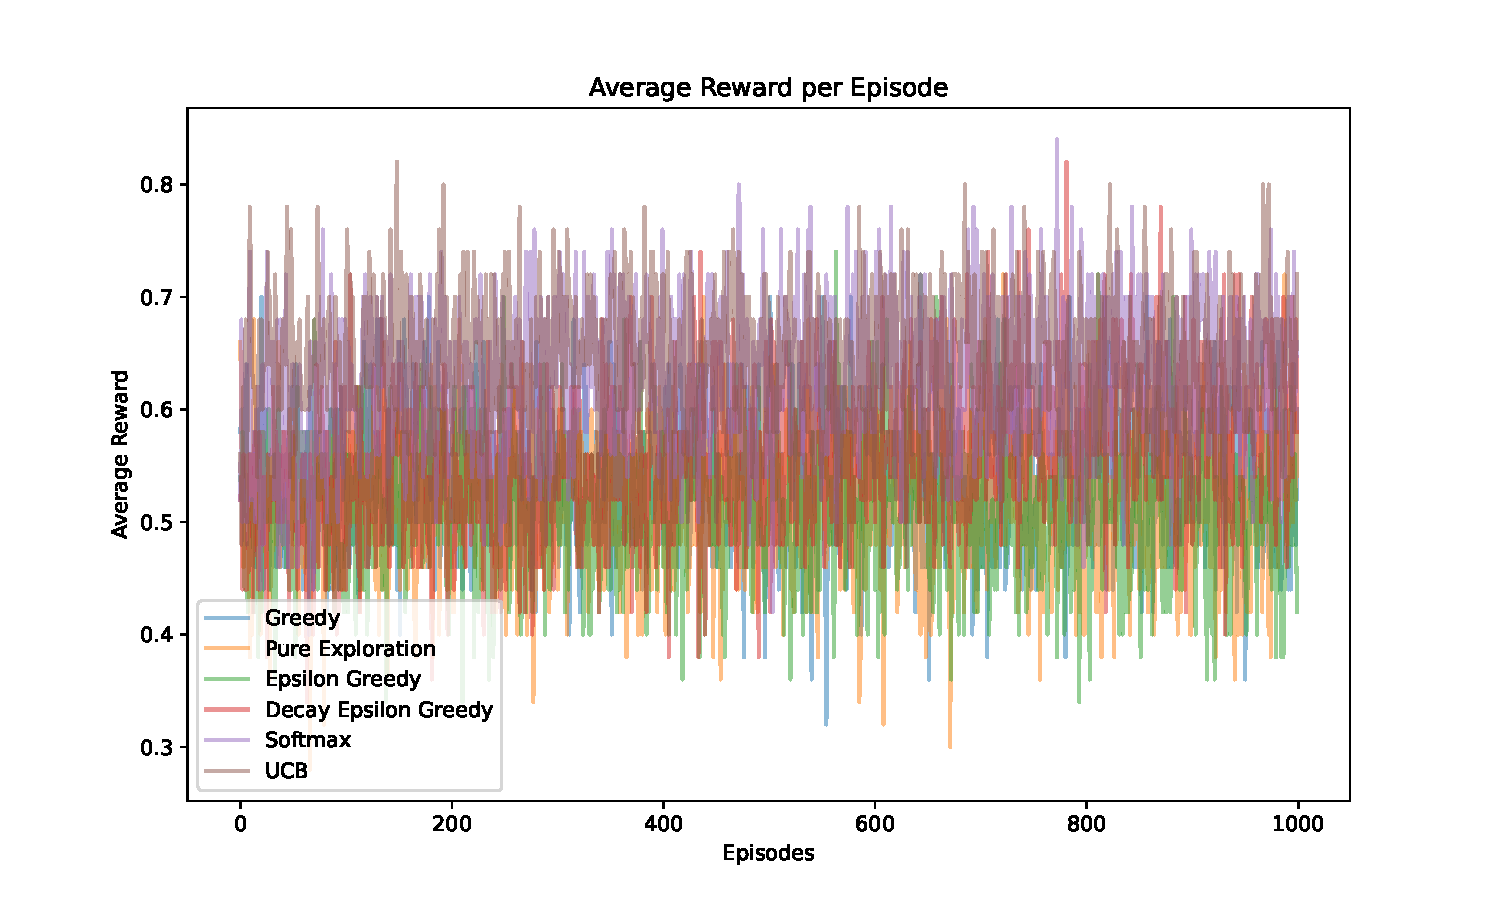
\includegraphics[width=\textwidth]{images/mab/bernoulli_average_reward_per_episode.pdf}
            \caption{Average reward}
            \label{fig:bernoulli_reward}
        \end{subfigure}

        \begin{subfigure}[b]{0.3\textwidth}
            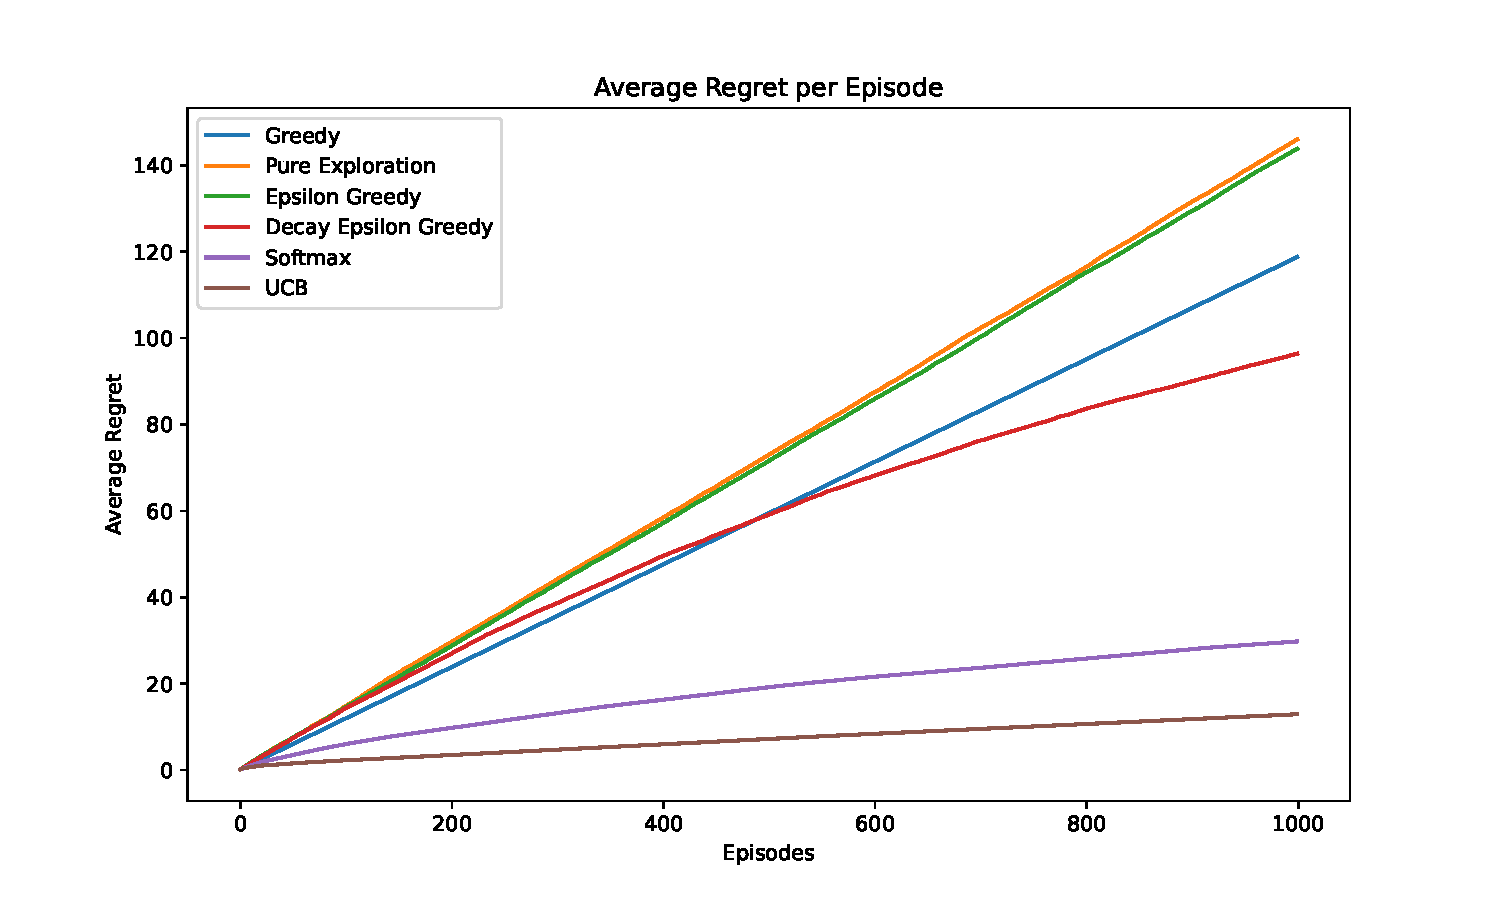
\includegraphics[width=\textwidth]{images/mab/bernoulli_average_regret_per_episode.pdf}
            \caption{Average regret}
            \label{fig:bernoulli_regret}
        \end{subfigure}

        \begin{subfigure}[b]{0.3\textwidth}
            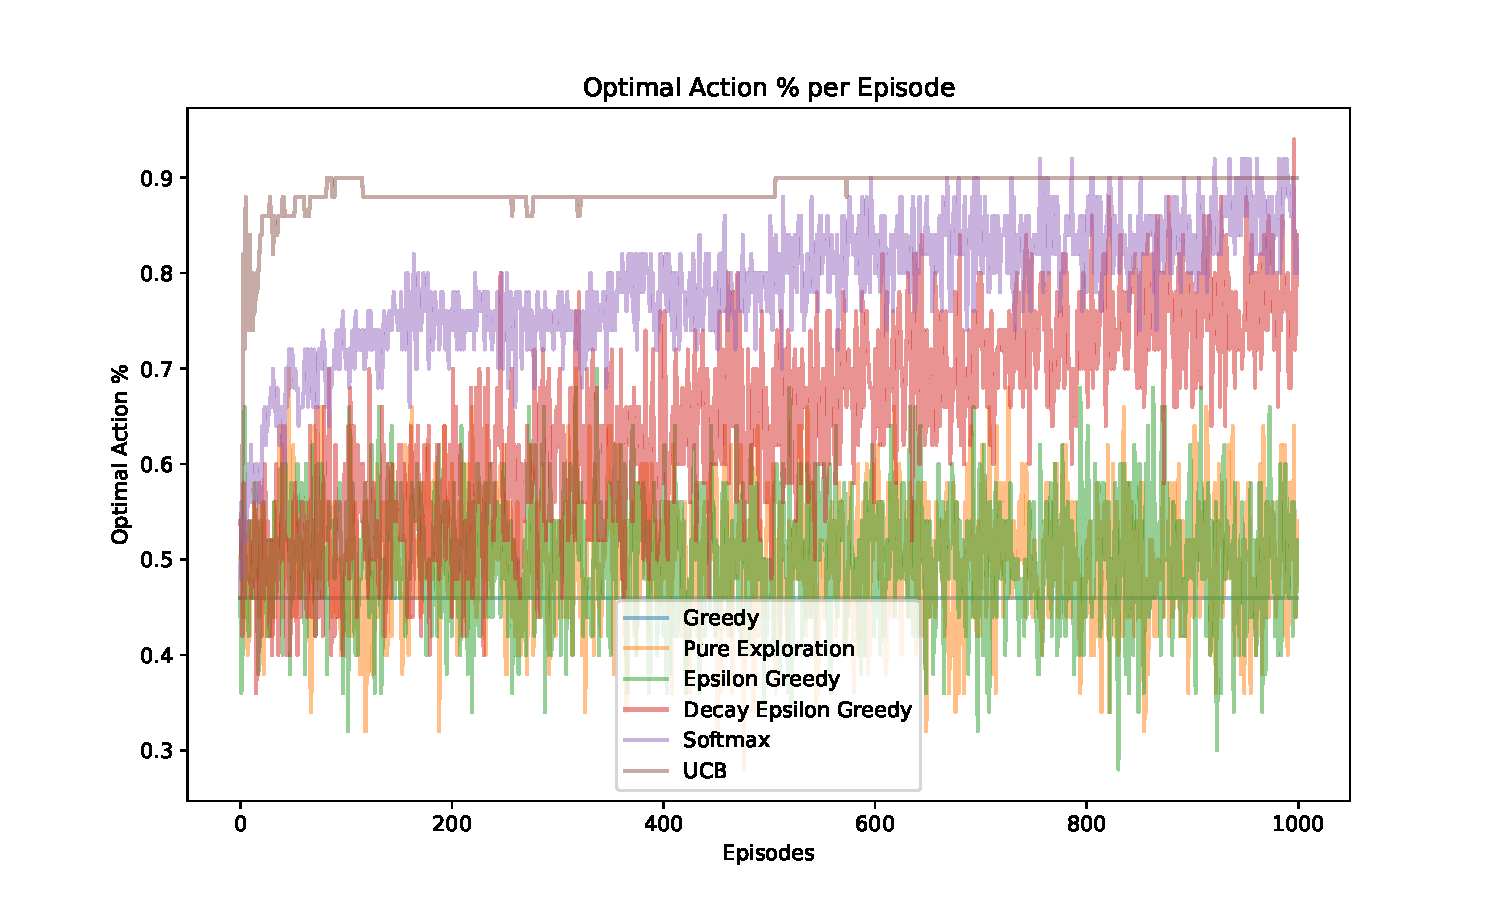
\includegraphics[width=\textwidth]{images/mab/bernoulli_optimal_actions_percentage_per_episode.pdf}
            \caption{Optimal Action \%}
            \label{fig:bernoulli_optimal_action}
        \end{subfigure}
        \caption{Results of 2-armed Bernoulli Bandit}

    \end{figure}

    \item Created a plot of the average regret of the agents for the 2-armed Bernoulli Bandit. Figure \ref{fig:bernoulli_regret} shows the average regret of the agents for the 2-armed Bernoulli Bandit. From the plot we can see that Greedy agent has the highest regret and it is continuously increasing. The epsilon-greedy and pure exploration agents have similar regret values. The regret of epsilon-decay rises as it is exploring but flattens out once it is confident about its environment. While the UBC and Softmax agents do not have much regret.
    

    \item Created a plot of the average regret of the agents for the 10-armed Gaussian Bandit. Figure \ref{fig:gaussian_regret} shows the average regret of the agents for the 10-armed Gaussian Bandit. From the plot we can see that Pure exploration leads to random reward retrivals making the agent gather more regret. The epsilon-greedy, epsilon-decay and UCB agents have similar regret values. While the greedy and softmax agents are very similar in regret values. We also notice that the regret does not sigificantly flatten out for any agent. Thus, we may need to run more steps to see the regret flatten out.
    \begin{figure}[h]
        \centering
        \begin{subfigure}[b]{0.3\textwidth}
            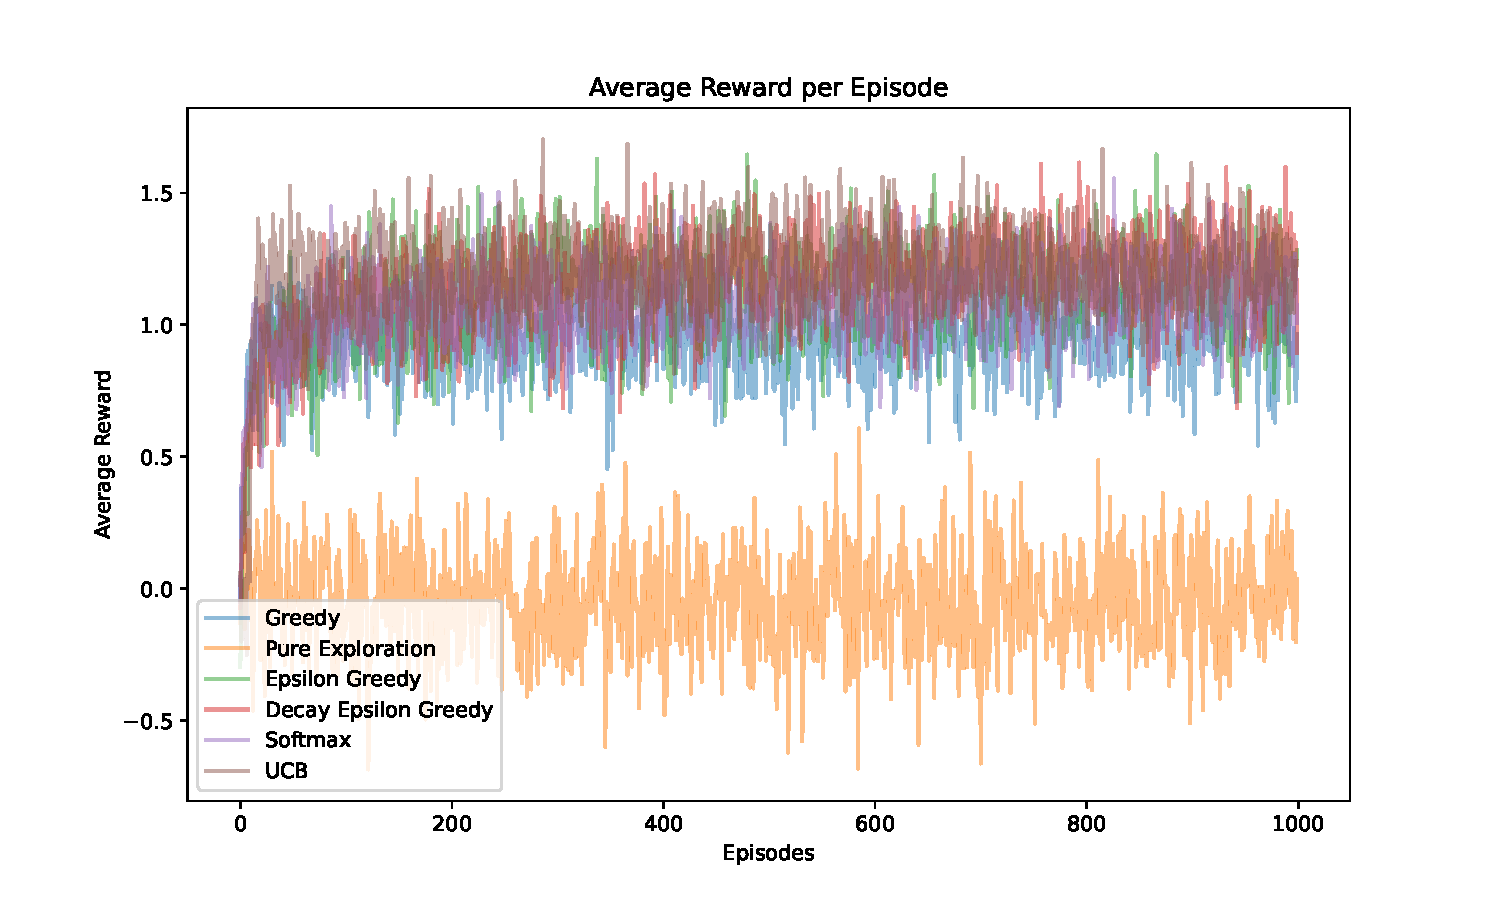
\includegraphics[width=\textwidth]{images/mab/10_arm_gaussian_average_reward_per_episode.pdf}
            \caption{Average reward}
            \label{fig:gaussian_reward}
        \end{subfigure}
        \begin{subfigure}[b]{0.3\textwidth}
            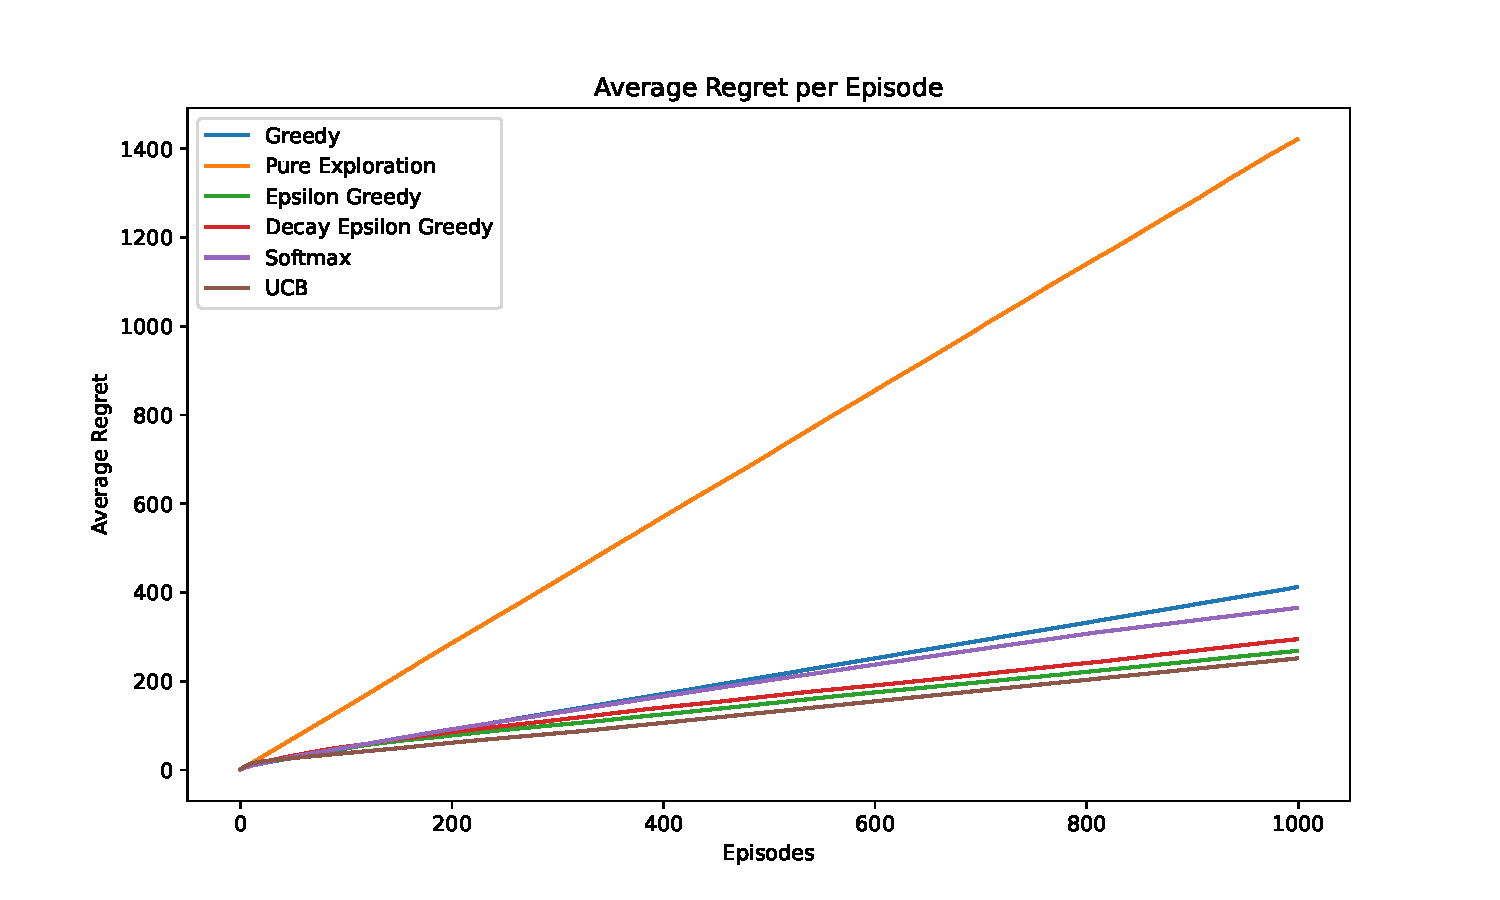
\includegraphics[width=\textwidth]{images/mab/10_arm_gaussian_average_regret_per_episode.pdf}
            \caption{Average regret}
            \label{fig:gaussian_regret}
        \end{subfigure}
        \begin{subfigure}[b]{0.3\textwidth}
            \centering
            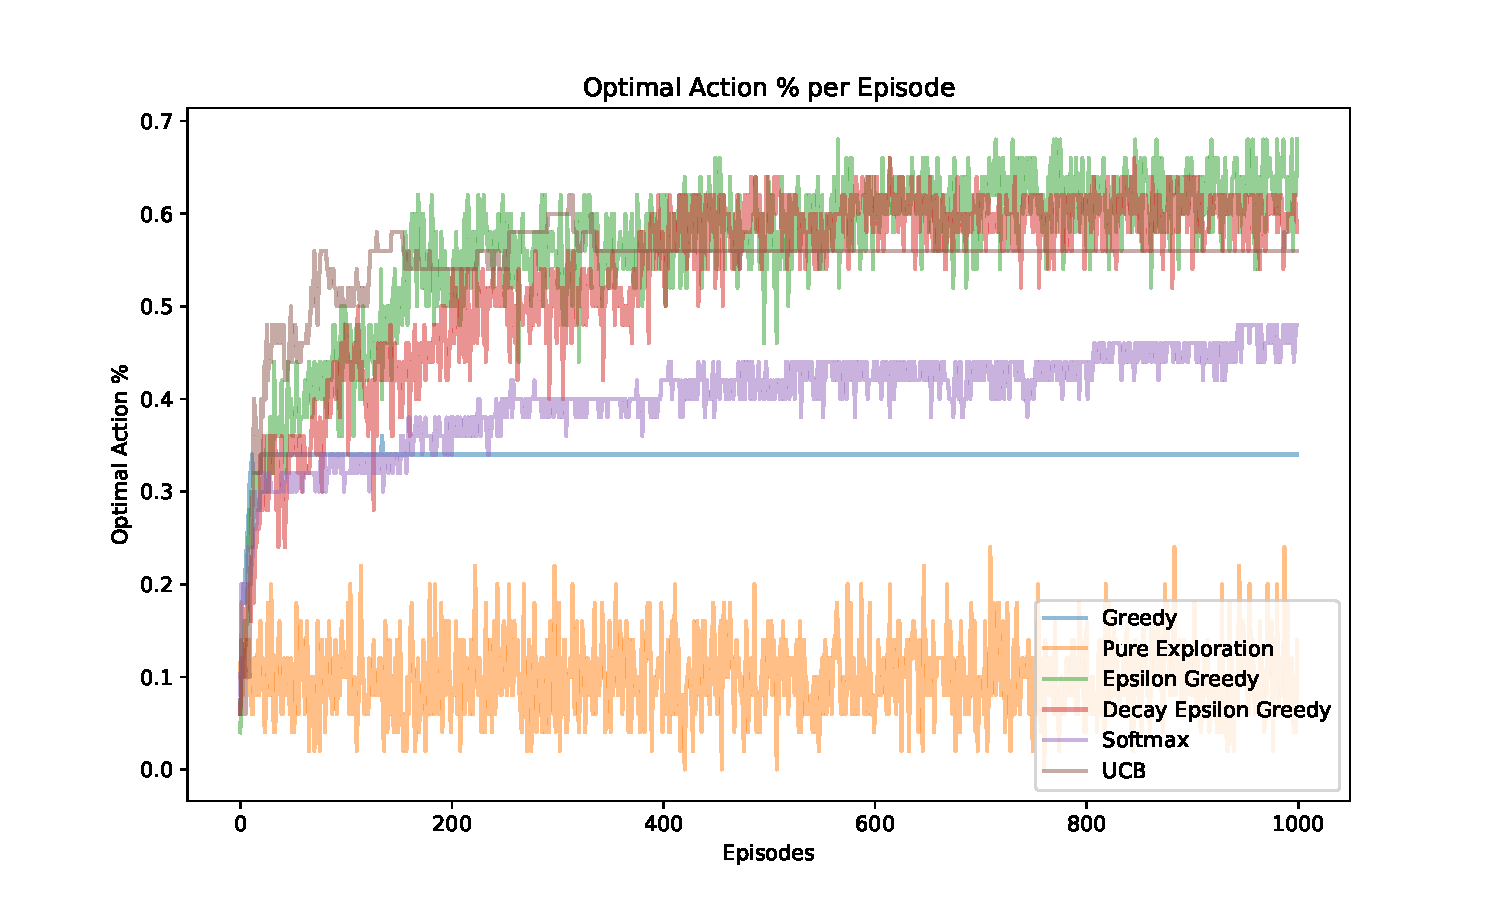
\includegraphics[width=\textwidth]{images/mab/10_arm_gaussian_optimal_actions_percentage_per_episode.pdf}
            \caption{Optimal Action \%}
            \label{fig:gaussian_optimal_action}
        \end{subfigure}
        \caption{Results of 10-armed Gaussian Bandit}
        
    \end{figure}

    \item This is the same as question 4. 
    
    \item Plotting the optimal action percentage of each agent for the 2-armed Bernoulli Bandit. Running 50 experiments did not reduce the variance by a noticeable margin, making the plots look very noisy. The results are shown in Figure \ref{fig:bernoulli_optimal_action}. From the plot we can see that the greedy agent has the lowest optimal action percentage. The epsilon-greedy and pure exploration agents have similar optimal action percentage, which means I have to change the eplison value even more. The UCB and Softmax agents have the highest optimal action percentage. While the epsilon-decay agent shows potential as its optimal action percentage increases with time. Running more expisodes could've proven the epsilon-decay agent to be the best.

    \item Plotting the optimal action percentage of each agent for the 10-armed Gaussian Bandit. The plots here are not as noisy as the 2-armed Bernoulli Bandit. The results are shown in Figure \ref{fig:gaussian_optimal_action}. From the plot we can see that the Pure exploration has the lowest optimal action percentage, which is inline with the regret plot of Pure exploration. This is followed by greedy and softmax agents. The optimal-action percentage plot shows that epsilon-greedy and epsilon-decay agents have the best action selection strategy and beat UCB agent by a noticeable margin, which is not evident from the regret plots.
    

\end{enumerate}
\Solution{2: MC Estimates and TD Learning}
\\

\noindent Code available at: \url{http://tinyurl.com/cs780-assignment-1-p2}

I started by implementing the \texttt{RandomWalk-v0} environment by subclassing the \texttt{gym.Env} class. The environment is a simple random walk with 7 states. The agent starts at the middle state and only moves left following the ``go-left'' policy. The agent terminates actions and receives a reward of $+1$ if it reaches the rightmost state and a reward of $0$ if it reaches the leftmost state. The agent receives a reward of $0$ on non-terminal states. The environment is completely stochastic and the agent has a probability of $0.5$ of moving left and right. The environment is working as expected, based on pygame observations and trajectory anaylsis.

We take the action space to be $\mathcal{A} = \{0, 1\}$ and the state space to be $\mathcal{S} = \{0, 1, 2, 3, 4, 5, 6\}$. Thus, to calculate the state-values, we can use the following equations:
\begin{align}
    V(s) = \mathbb{E}[G_t|S_t=s] &= \mathbb{E}[R_{t+1} + \gamma G_{t+1}|S_t=s] \\
    &= \sum_{a}\pi(a|s)\sum_{s^{\prime}, r}p(s^{\prime}, r| s, a)[r + \gamma V(s^{\prime})]
\end{align}
We can now fill in values for each of the variables and calculate the state-values. As there is only 1 action we choose for each state (following a predetermined policy $\pi=$``go left''), we can ignore the $\pi(a|s)$ term.
\begin{align*}
    v(0) &= 0 \\
    v(1) &= p(0, 0|1, 0)[0 + \gamma v(0)] + p(2, 0|1, 0)[0 + \gamma v(2)] \\
    v(2) &= p(1, 0|2, 0)[0 + \gamma v(1)] + p(3, 0|2, 0)[0 + \gamma v(3)] \\
    v(3) &= p(2, 0|3, 0)[0 + \gamma v(2)] + p(4, 0|3, 0)[0 + \gamma v(4)] \\
    v(4) &= p(3, 0|4, 0)[0 + \gamma v(3)] + p(5, 0|4, 0)[0 + \gamma v(5)] \\
    v(5) &= p(4, 0|5, 0)[0 + \gamma v(4)] + p(6, 1|5, 0)[1 + \gamma v(6)] \\
    v(6) &= 0 \\
\end{align*}

Upon rearranging the terms we get:
\begin{align*}
    v(0) &= 0 \\
    v(1) - \frac{\gamma}{2}v(2) &= 0 \\
    v(2) - \frac{\gamma}{2}v(1) - \frac{\gamma}{2}v(3) &= 0 \\
    v(3) - \frac{\gamma}{2}v(2) - \frac{\gamma}{2}v(4) &= 0 \\
    v(4) - \frac{\gamma}{2}v(3) - \frac{\gamma}{2}v(5) &= 0 \\
    v(5) - \frac{\gamma}{2}v(4) &= \frac{1}{2} \\
    v(6) &= 0 \\
\end{align*}

Rewriting the above equations in matrix form we get:
\begin{align*}
    \begin{bmatrix}
        1 & -\frac{\gamma}{2} & 0 & 0 & 0 \\
        -\frac{\gamma}{2} & 1 & -\frac{\gamma}{2} & 0 & 0 \\
        0 & -\frac{\gamma}{2} & 1 & -\frac{\gamma}{2} & 0 \\
        0 & 0 & -\frac{\gamma}{2} & 1 & -\frac{\gamma}{2} \\
        0 & 0 & 0 & -\frac{\gamma}{2} & 1 \\
    \end{bmatrix}
    \begin{bmatrix}
        v(1) \\
        v(2) \\
        v(3) \\
        v(4) \\
        v(5) \\
    \end{bmatrix}
    &=
    \begin{bmatrix}
        0 \\
        0 \\
        0 \\
        0 \\
        \frac{1}{2} \\
    \end{bmatrix}
\end{align*}
Solving the above for $\gamma=0.99$ we get:
\begin{align*}
    v(1) = 0.1501; 
    v(2) = 0.3032; 
    v(3) = 0.4624; 
    v(4) = 0.6310; 
    v(5) = 0.8124
\end{align*}

In all the below test cases and scenarios a seed of $21$ is used. I have also added \texttt{CONFIG} dictionary at any code block which is producing an output to be able to change values and observe outputs.
\begin{enumerate}
    
    \item I created a function \texttt{generate\_episode\_trajectory(environment, config=None)} which takes in the \texttt{environment} and a \texttt{config} dictionary and returns a list of tuples of the form $(s, a, r, s^{\prime})$. I tested the function with the \texttt{RandomWalk-v0} environment and the trajectory is as expected. The trajectory is shown in the code block below.
    \begin{verbatim}
Episode Trajectory: [(3, 0, 0.0, 2), (2, 0, 0.0, 3), (3, 0, 0.0, 4), 
(4, 0, 0.0, 3), (3, 0, 0.0, 2), (2, 0, 0.0, 3), (3, 0, 0.0, 4), 
(4, 0, 0.0, 5), (5, 0, 1.0, 6)]
    \end{verbatim}
    
    \item I wrote a routine to decay the step size at every step/episode: \texttt{decay\_step\_size(initial\_value, final\_value, episode, max\_episode, decay\_type, decay\_stop=None)}. This routine returns $\alpha(e)$ which starts at \texttt{initial\_value} and ends at \texttt{final\_value} based on the \texttt{decay\_type}. I tested the function and the results are present in Figure \ref{fig:exp_step_size_decay} and Figure \ref{fig:linear_step_size_decay}. The step size is decaying as expected.
    \begin{figure}[h]
        \centering
        \begin{subfigure}[b]{0.45\textwidth}
            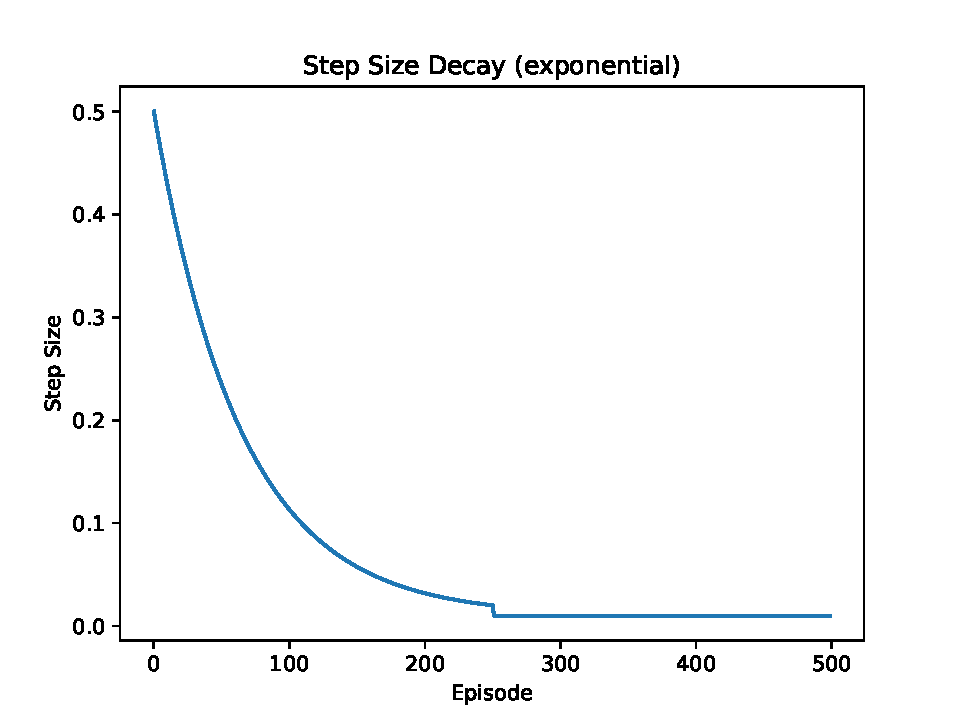
\includegraphics[width=\textwidth]{images/mc_td/step_size_decay_exponential.pdf}
            \caption{Exponential}
            \label{fig:exp_step_size_decay}
        \end{subfigure}
        \begin{subfigure}[b]{0.45\textwidth}
            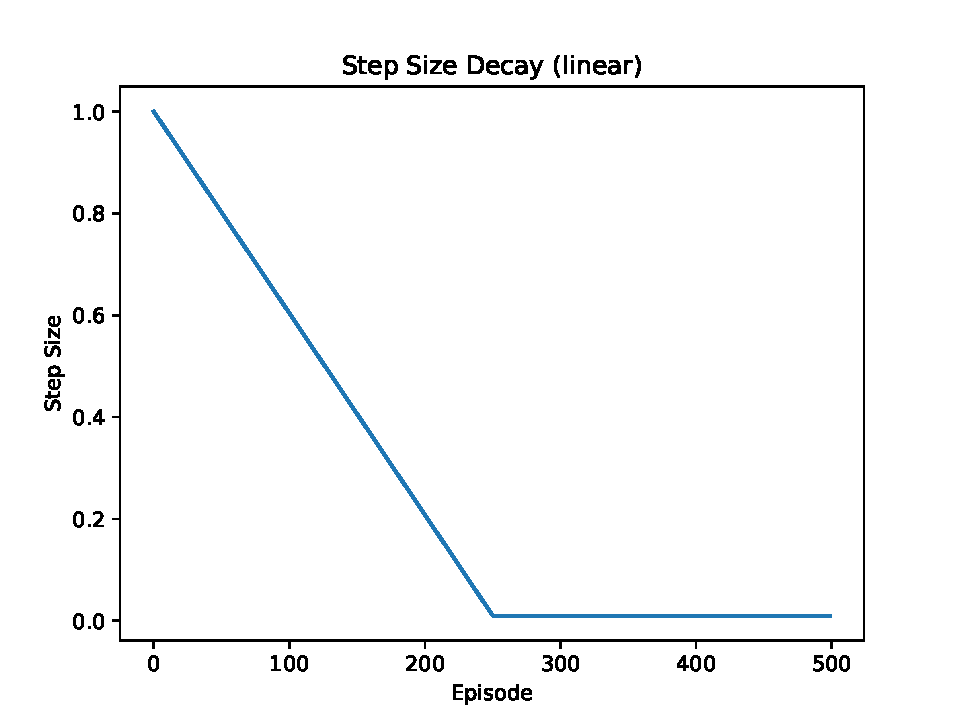
\includegraphics[width=\textwidth]{images/mc_td/step_size_decay_linear.pdf}
            \caption{Linear}
            \label{fig:linear_step_size_decay}
        \end{subfigure}
        \caption{Exponential and Linear decay of step-size for 500 steps, initial value=$0.5$, final value=$0.01$ and decrease only till step $250$ after which it remains constant}
    \end{figure}

    \item I implemented a routine to run Monte Carlo prediction for first-visit and every-visit scenarios. This is again controlled by \texttt{CONFIG} parameter. Below is an output from the routine for first-visit Monte Carlo prediction. The output consists of the state values, state-values for all episodes and the trajectory of the agent.
    \begin{verbatim}
(array([0., 0., 0., 0., 0., 0., 0.]),
array([[0., 0., 0., 0., 0., 0., 0.]]),
[(3, 0, 0.0, 2), (2, 0, 0.0, 1), (1, 0, 0.0, 0)])
    \end{verbatim}

    \item I implemented a routine to run Temporal difference prediction. This routine like the above not only does prediction but also computes the state-values. This is again controlled by \texttt{CONFIG} parameter. Below is an output from the routine for TD prediction routine. The output consists of the state values, state-values for all episodes and the trajectory of the agent.
    \begin{verbatim}
(array([0. , 0. , 0. , 0. , 0. , 0.1, 0. ]),
array([[0. , 0. , 0. , 0. , 0. , 0.1, 0. ]]),
[(3, 0, 0.0, 2), (2, 0, 0.0, 1), (1, 0, 0.0, 0)])
    \end{verbatim}
    \item I wrote a routine to plot the state-values across episodes and $log($episodes$)$ to answer multiple questions below. \texttt{plot\_episode\_values(V\_r, image\_name, config=None)} takes the state-values across episodes along with an \texttt{image\_name} to save the image and a \texttt{config} for additional information.

    I plotted the state-values for each state for First-Visit MC in Figure \ref{fig:default_fvmc} and \ref{fig:tuned_fvmc}. We can see from the from the figures that there is initially very high variance in the state-values but as the number of episodes increase the variance decreases and the state-values converge to the true values. The variance is higher in the default case as the step size is too high and the decay is too slow. The variance is lower in the tuned case as the step size is lower and the final value is also very low. On the log-scale plot, we can see that the state-values slowly rise towards the true values.

    \begin{figure}[h]
        \centering
        \begin{subfigure}[b]{0.8\textwidth}
            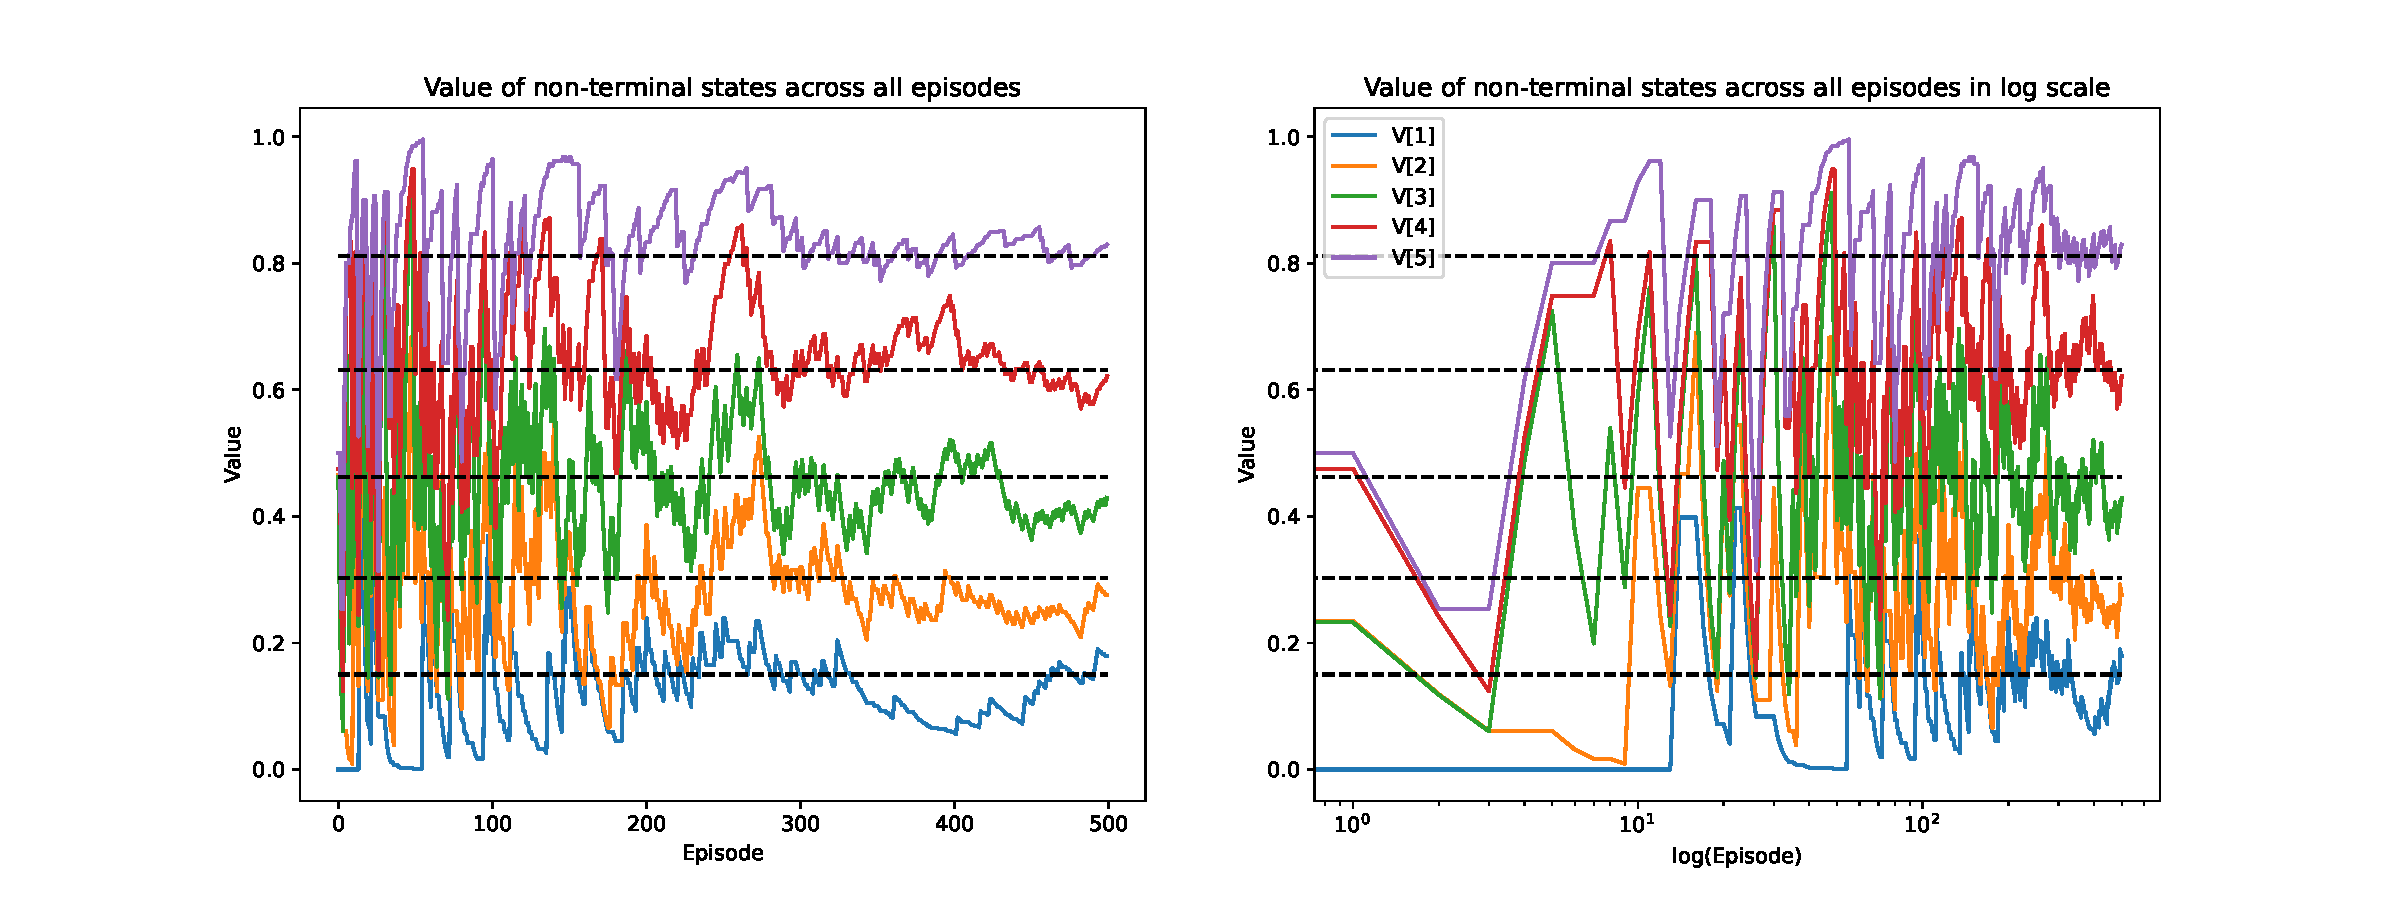
\includegraphics[width=\textwidth]{images/mc_td/first_visit_exponential_0.5_0.01_episode_values.pdf}
            \caption{Exponential decay of step size}
            \label{fig:default_fvmc}
        \end{subfigure}

        \begin{subfigure}[b]{0.8\textwidth}
            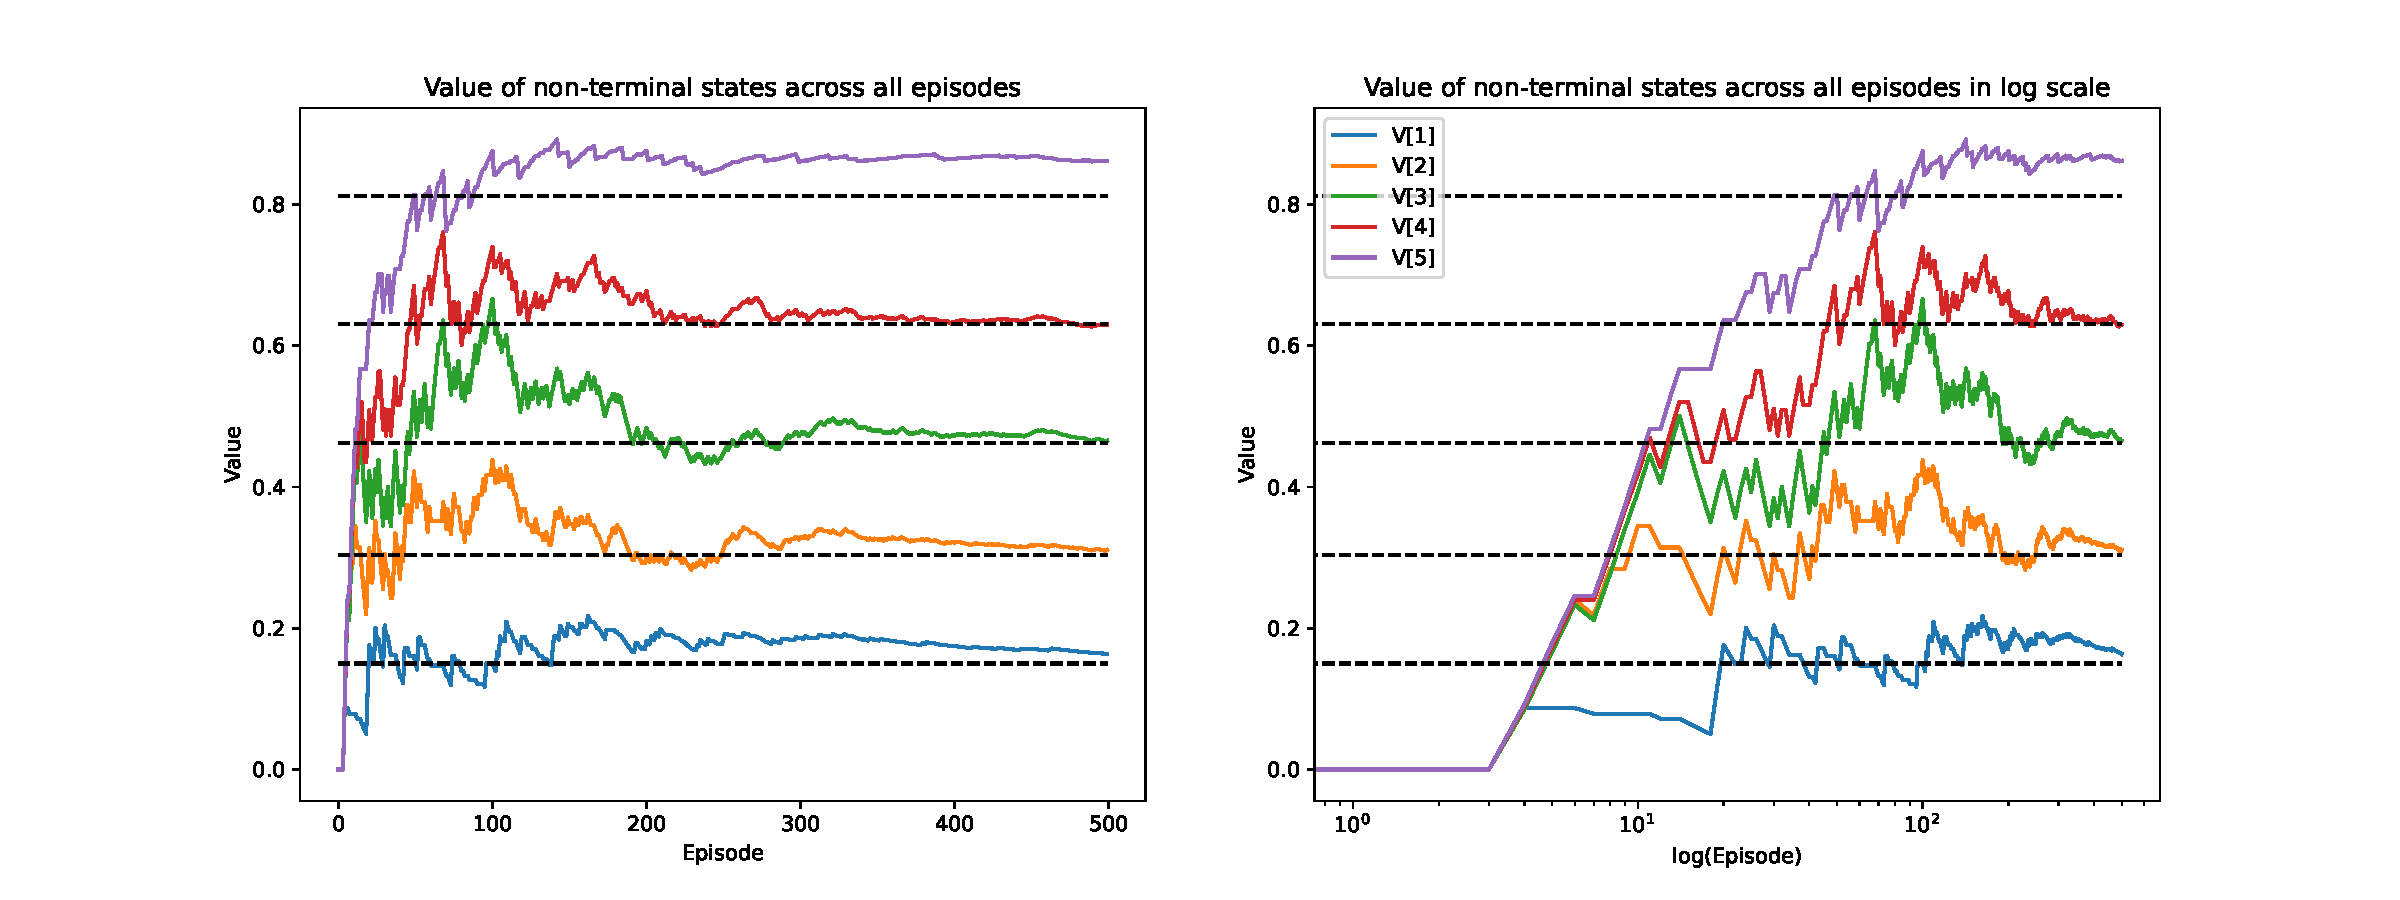
\includegraphics[width=\textwidth]{images/mc_td/first_visit_exponential_0.1_0.0008_episode_values.pdf}
            \caption{Exponential decay and tuned hyperparameters}
            \label{fig:tuned_fvmc}
        \end{subfigure}
        \caption{First-Visit MC}
    \end{figure}

    \item I plotted the state-values for each state for Every-Visit MC in Figure \ref{fig:default_evmc} and \ref{fig:tuned_evmc}. We can see from the from the figures that there is initially very high variance in the state-values but as the number of episodes increase the variance decreases and the state-values converge to the true values. The variance is higher in the default case as the step size is too high and the decay is too slow. I then tuned the hyperparameters and the variance is lower in the tuned case as the step size is lower and the final value is also very low, while achieving very low bias on the true values. On the log-scale plot, we can make a better judgement on the high variance phenomenon of Monte Carlo methods.
    \begin{figure}[h]
        \centering
        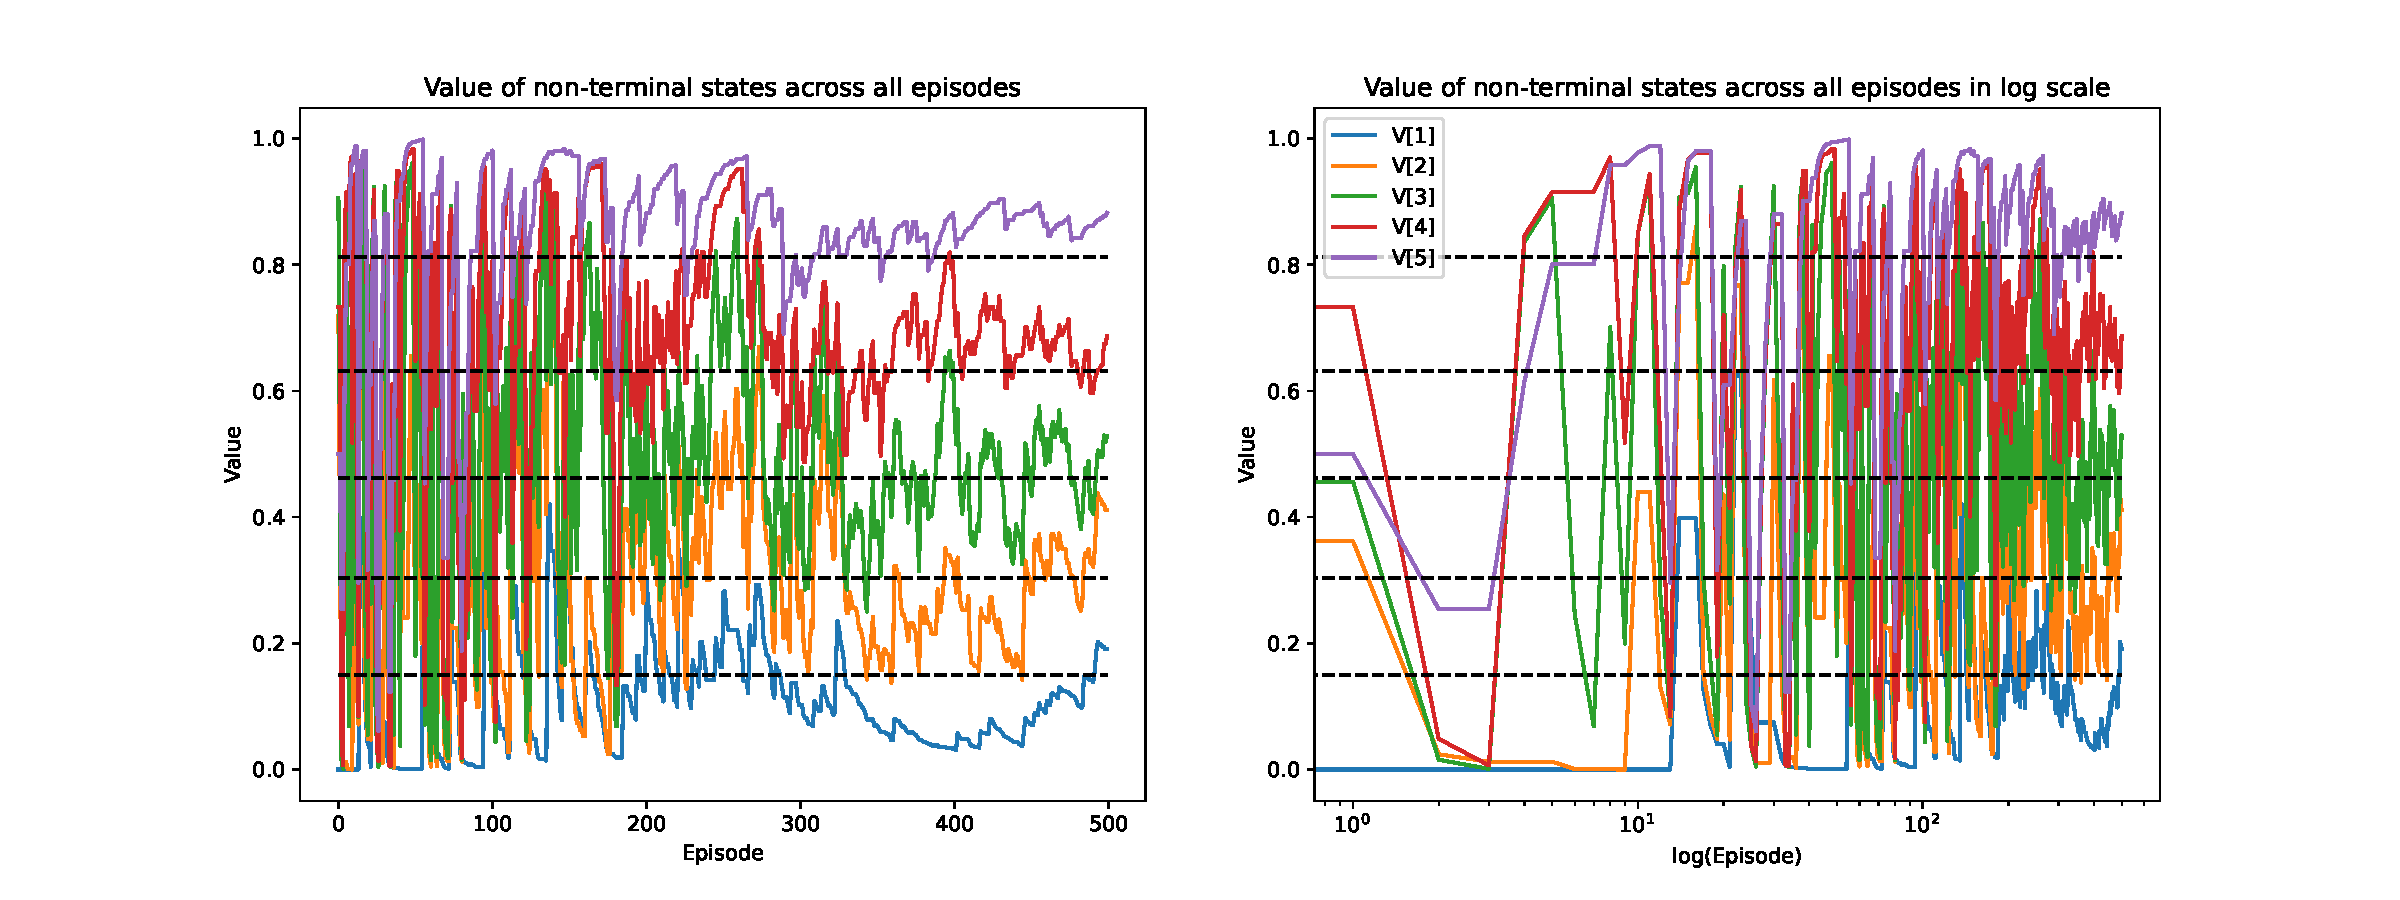
\includegraphics[width=\textwidth]{images/mc_td/every_visit_exponential_0.5_0.01_episode_values.pdf}
        \caption{EVMC with exponential decay of step size}
        \label{fig:default_evmc}
    \end{figure}

    \begin{figure}[h]
        \centering
        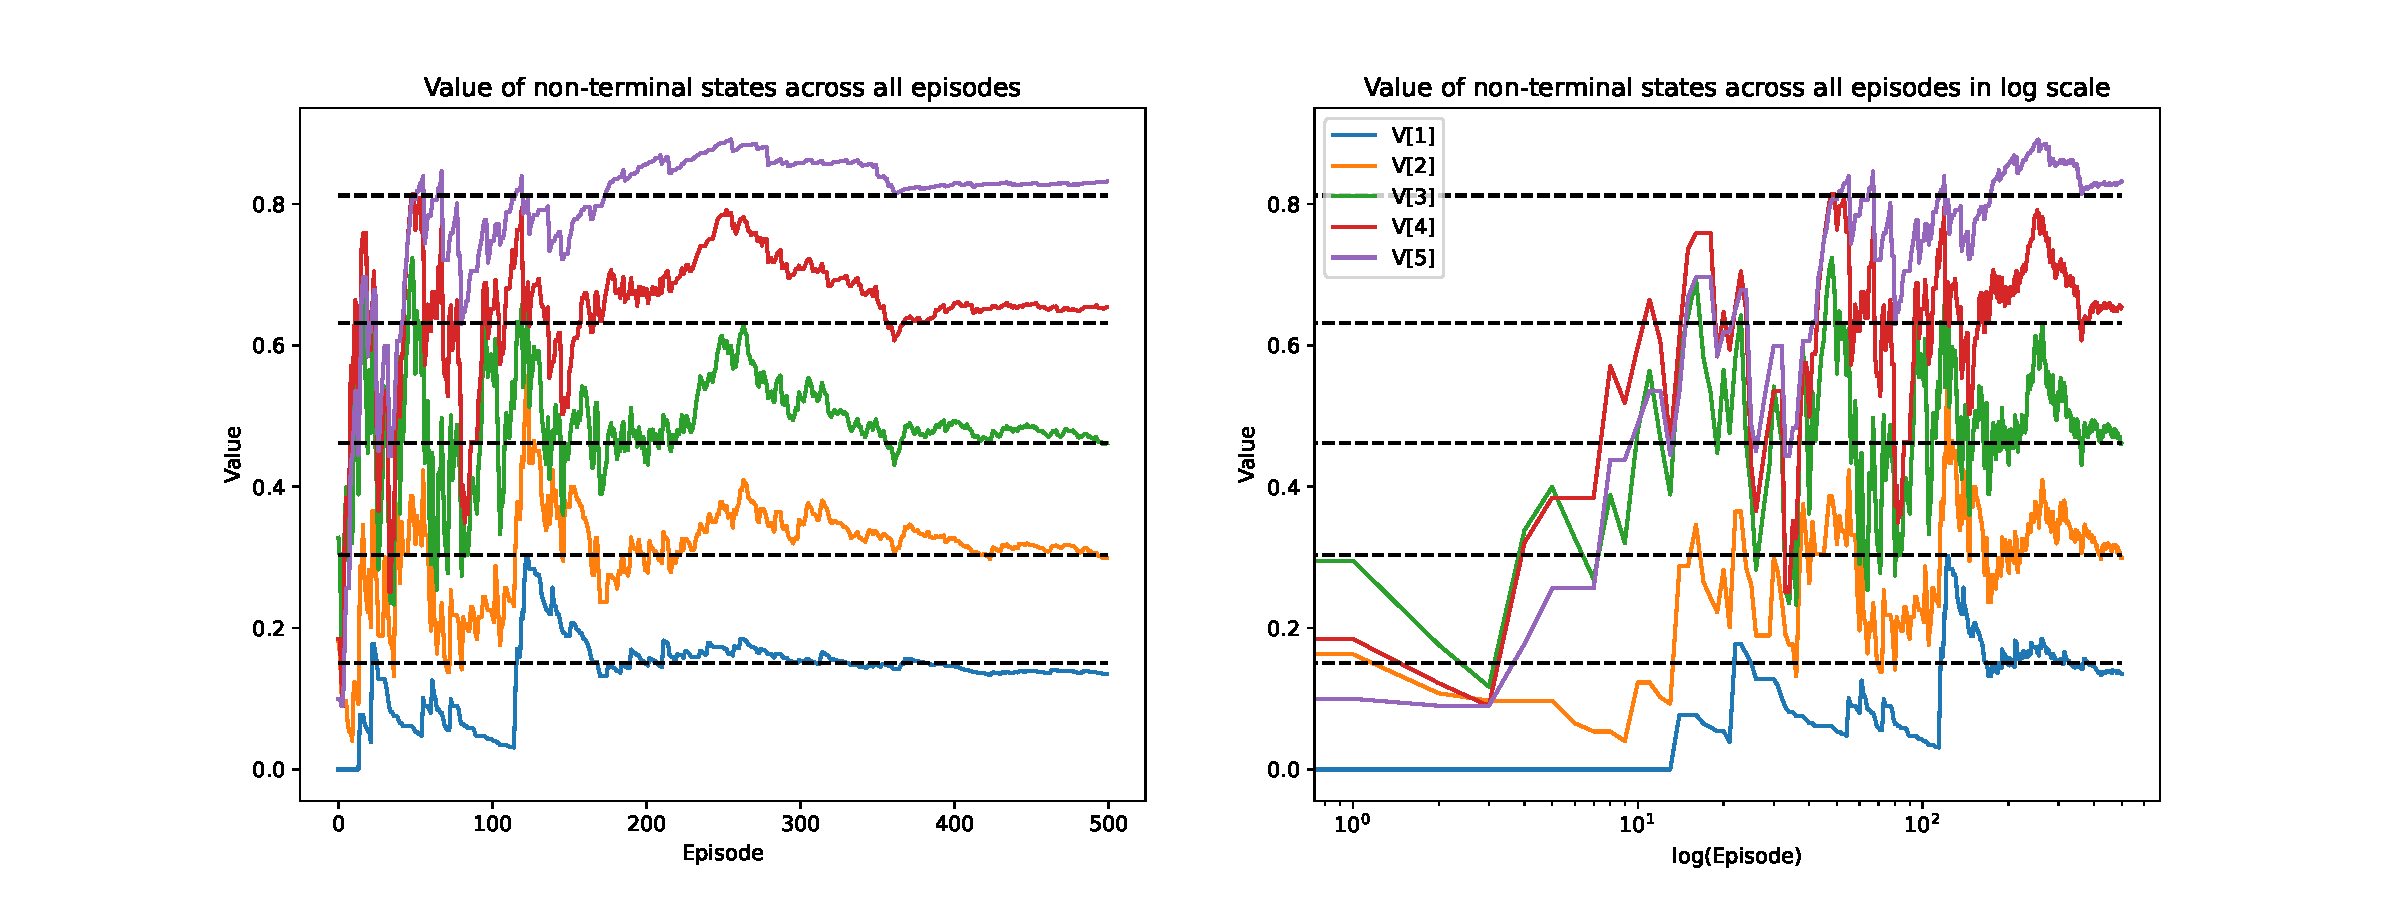
\includegraphics[width=\textwidth]{images/mc_td/every_visit_exponential_0.1_0.0008_episode_values.pdf}
        \caption{EVMC with exponential decay and tuned hyperparameters}
        \label{fig:tuned_evmc}
    \end{figure}

    \item I plotted the state-values for each state for TD prediction in Figure \ref{fig:default_td} and \ref{fig:tuned_td}. Before and after tuning we can observe that the variance in all the state-values of TD are low but the state-values never seem to converge at the true values. This shows the high bias TD learning has, as discussed in class.
    \begin{figure}[h]
        \centering
        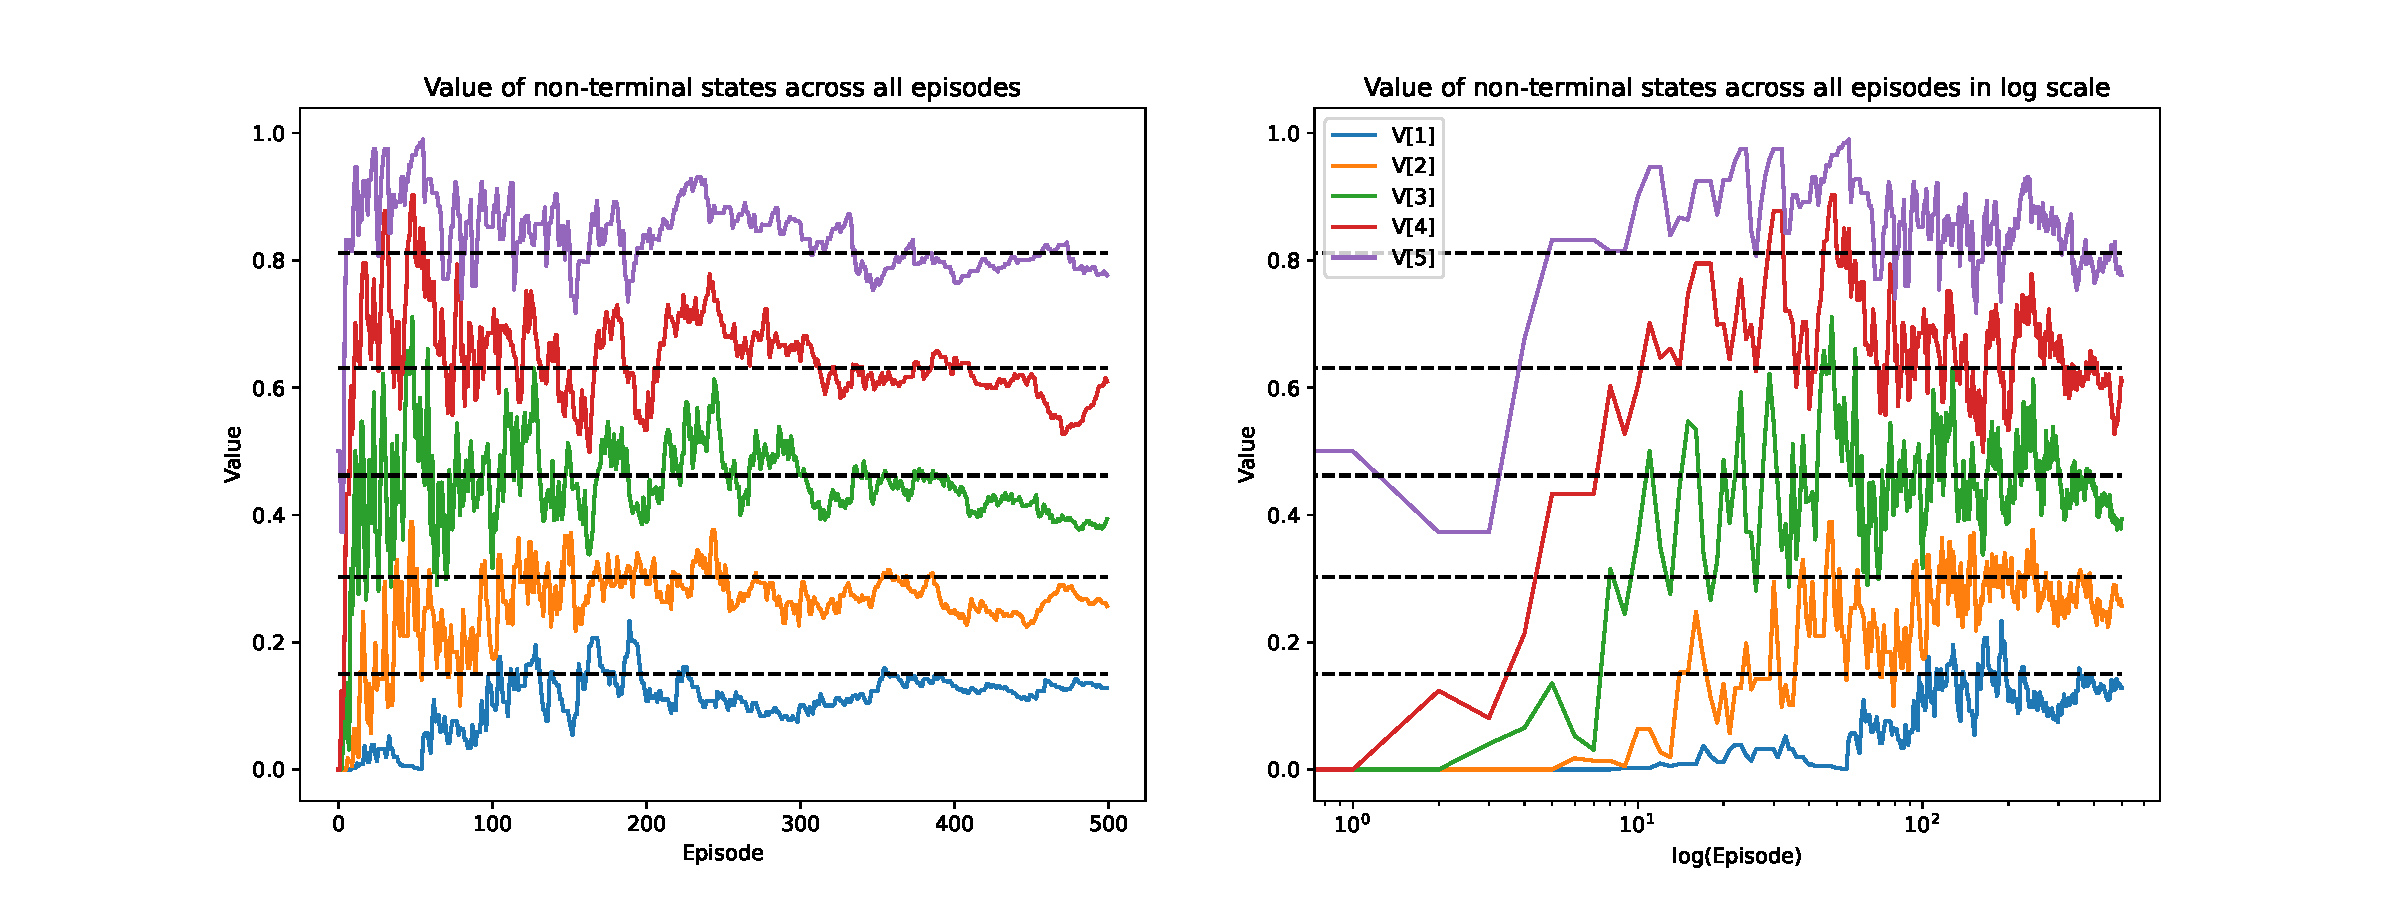
\includegraphics[width=\textwidth]{images/mc_td/td_learning_exponential_0.5_0.01_episode_values.pdf}
        \caption{TD with exponential decay of step size}
        \label{fig:default_td}
    \end{figure}

    \begin{figure}[h]
        \centering
        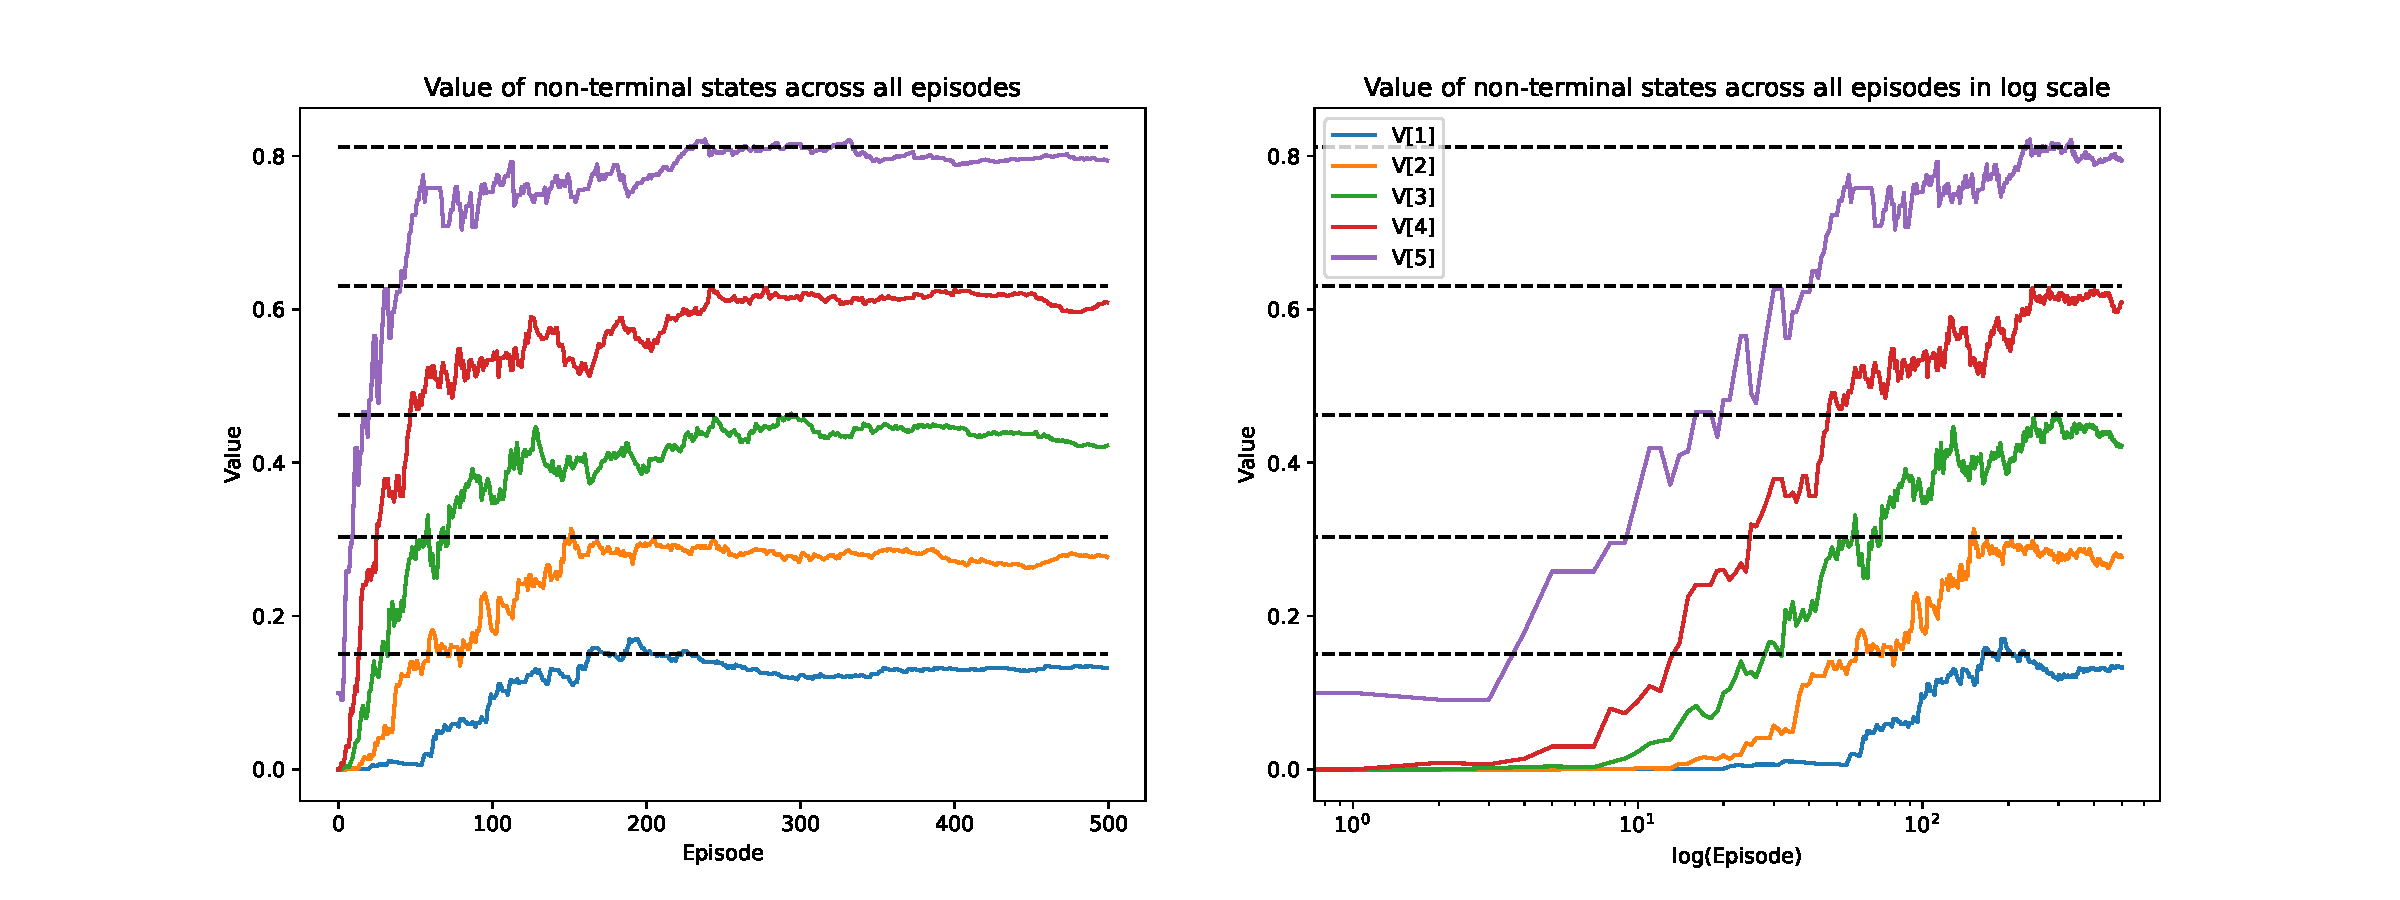
\includegraphics[width=\textwidth]{images/mc_td/td_learning_exponential_0.1_0.002_episode_values.pdf}
        \caption{TD with exponential decay and tuned hyperparameters}
        \label{fig:tuned_td}
    \end{figure}

    \item In this question I wrote a routine to run experiments for \texttt{max\_runs} number of times. The routine runs First-Visit MC, Every-Visit MC and TD learning for \texttt{max\_episodes} number of episodes using the tuned hyperparameters for each of the algorithms. The routine then plots the average state-values across all runs for each algorithm. The results are shown in Figure \ref{fig:average_fvmc}, \ref{fig:average_evmc} and \ref{fig:average_td}. We can see that the average state-values for First-Visit MC and Every-Visit MC converge to the true values but the average state-values for TD learning do not converge to the true values. This is consistent with the general behaviours of the algorithms.
    \begin{figure}[h]
        \centering
        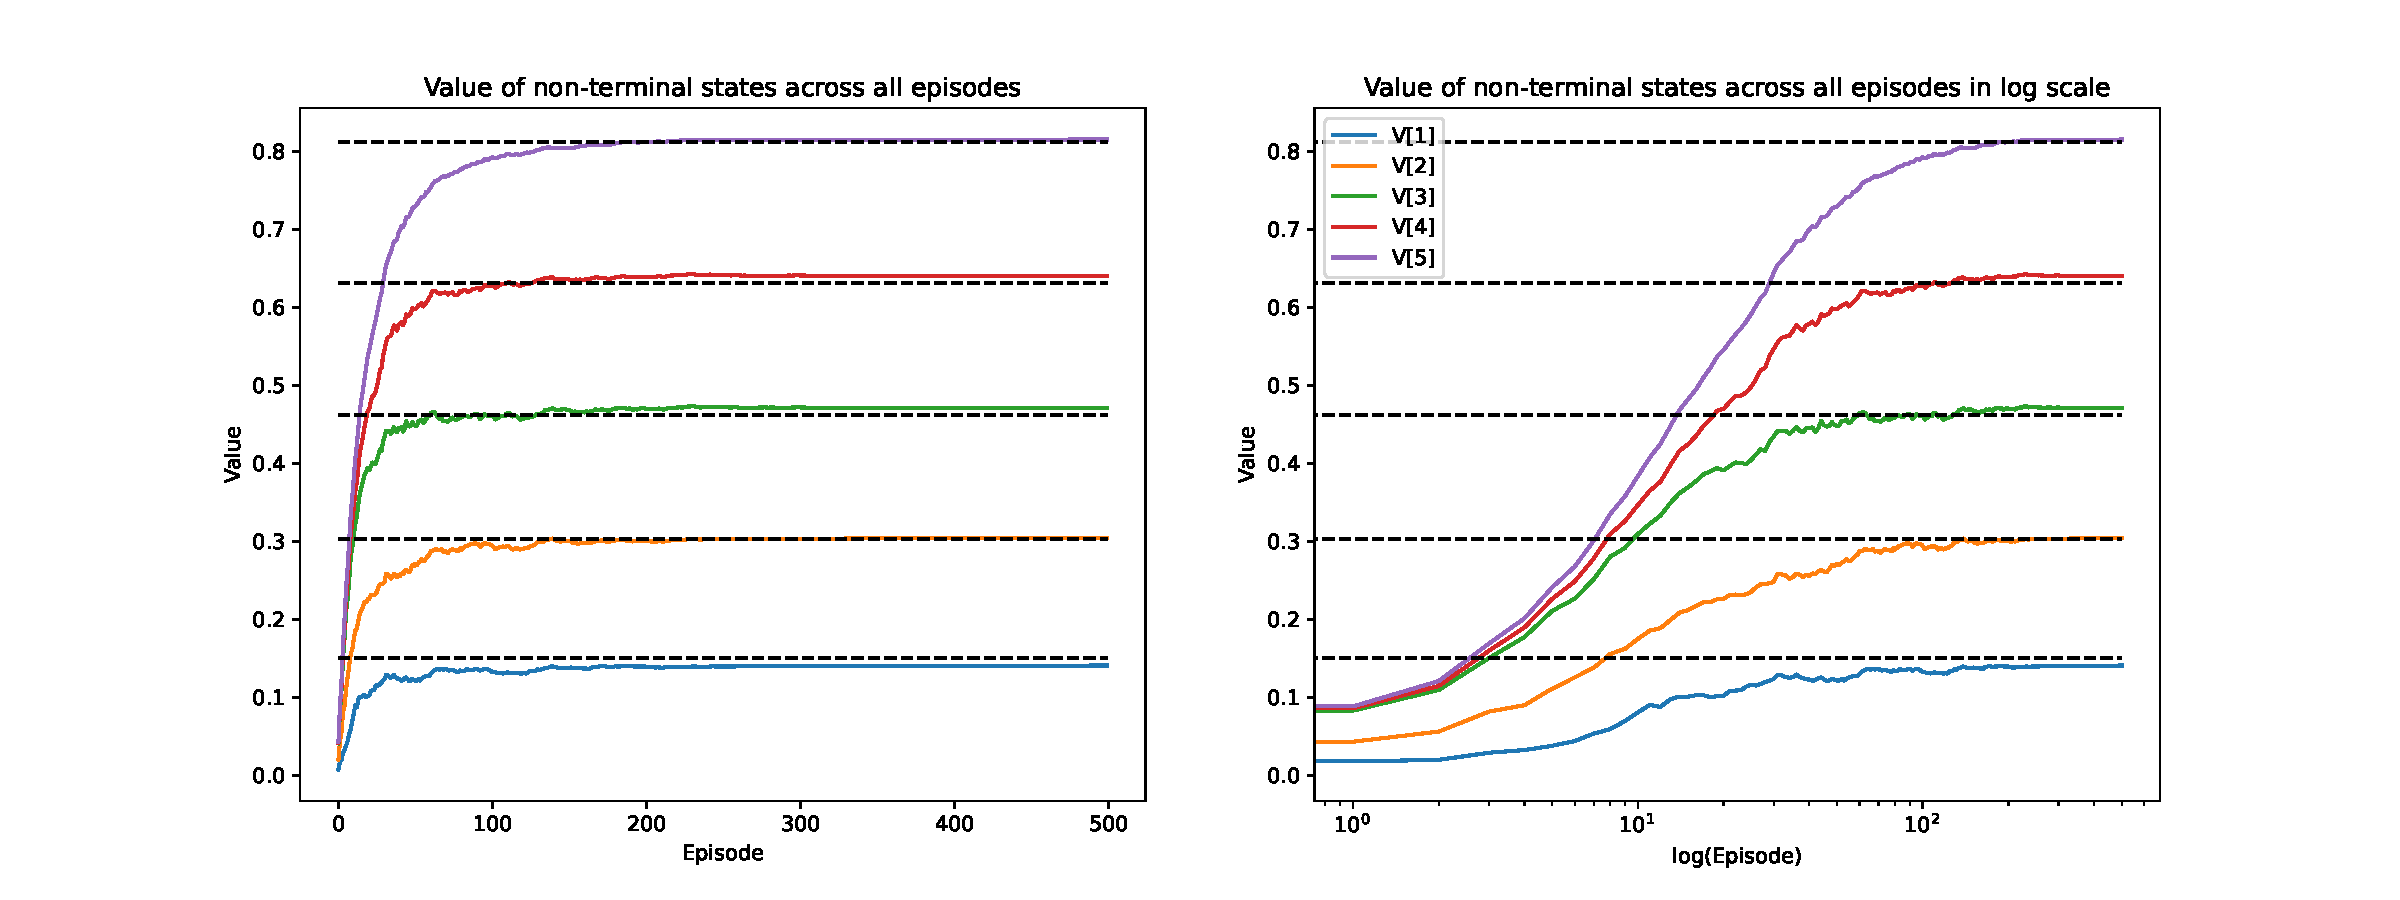
\includegraphics[width=\textwidth]{images/mc_td/fvmc_experiments_50.pdf}
        \caption{Average state-values of 50 runs of FVMC with exponential decay and tuned hyperparameters}
        \label{fig:average_fvmc}
    \end{figure}

    \begin{figure}[h]
        \centering
        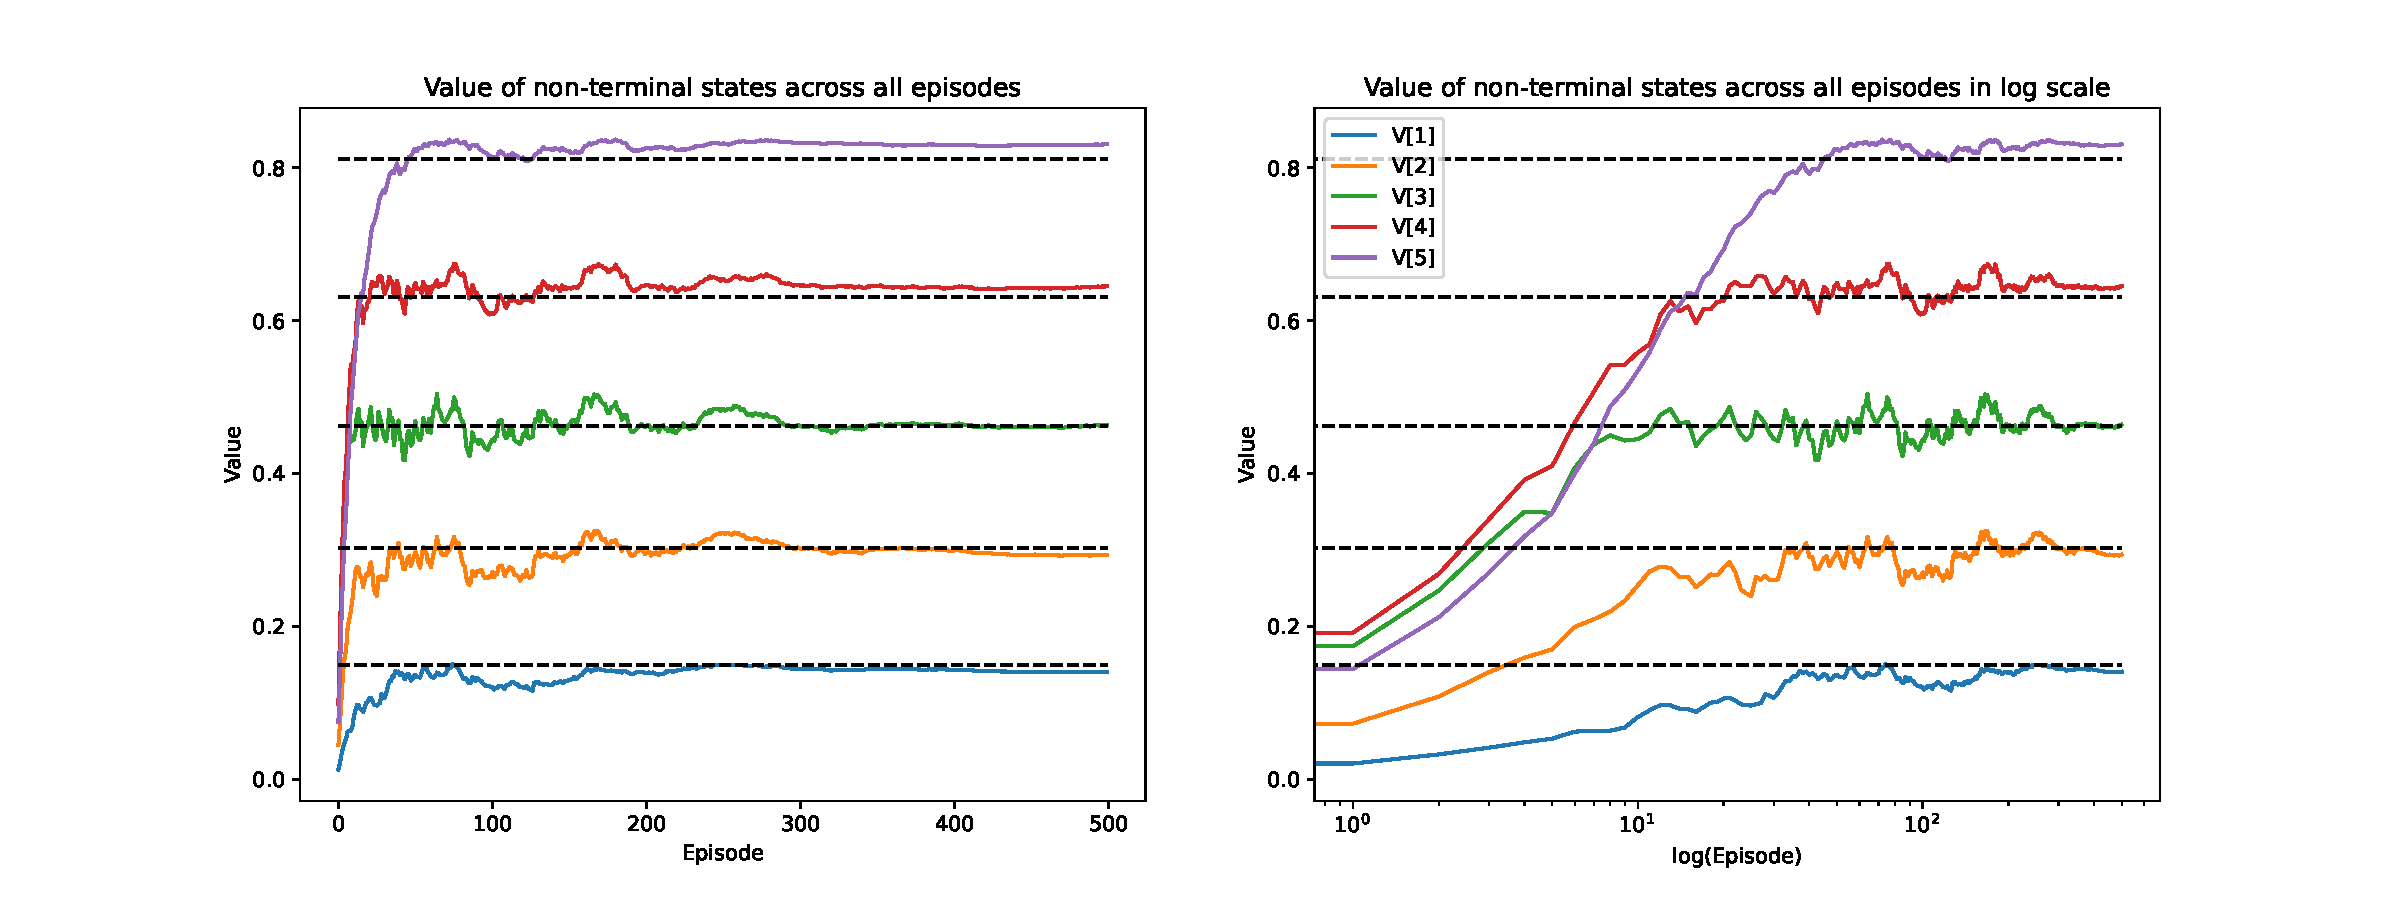
\includegraphics[width=\textwidth]{images/mc_td/evmc_experiments_50.pdf}
        \caption{Average state-values of 50 runs of EVMC with exponential decay and tuned hyperparameters}
        \label{fig:average_evmc}
    \end{figure}

    \begin{figure}[h]
        \centering
        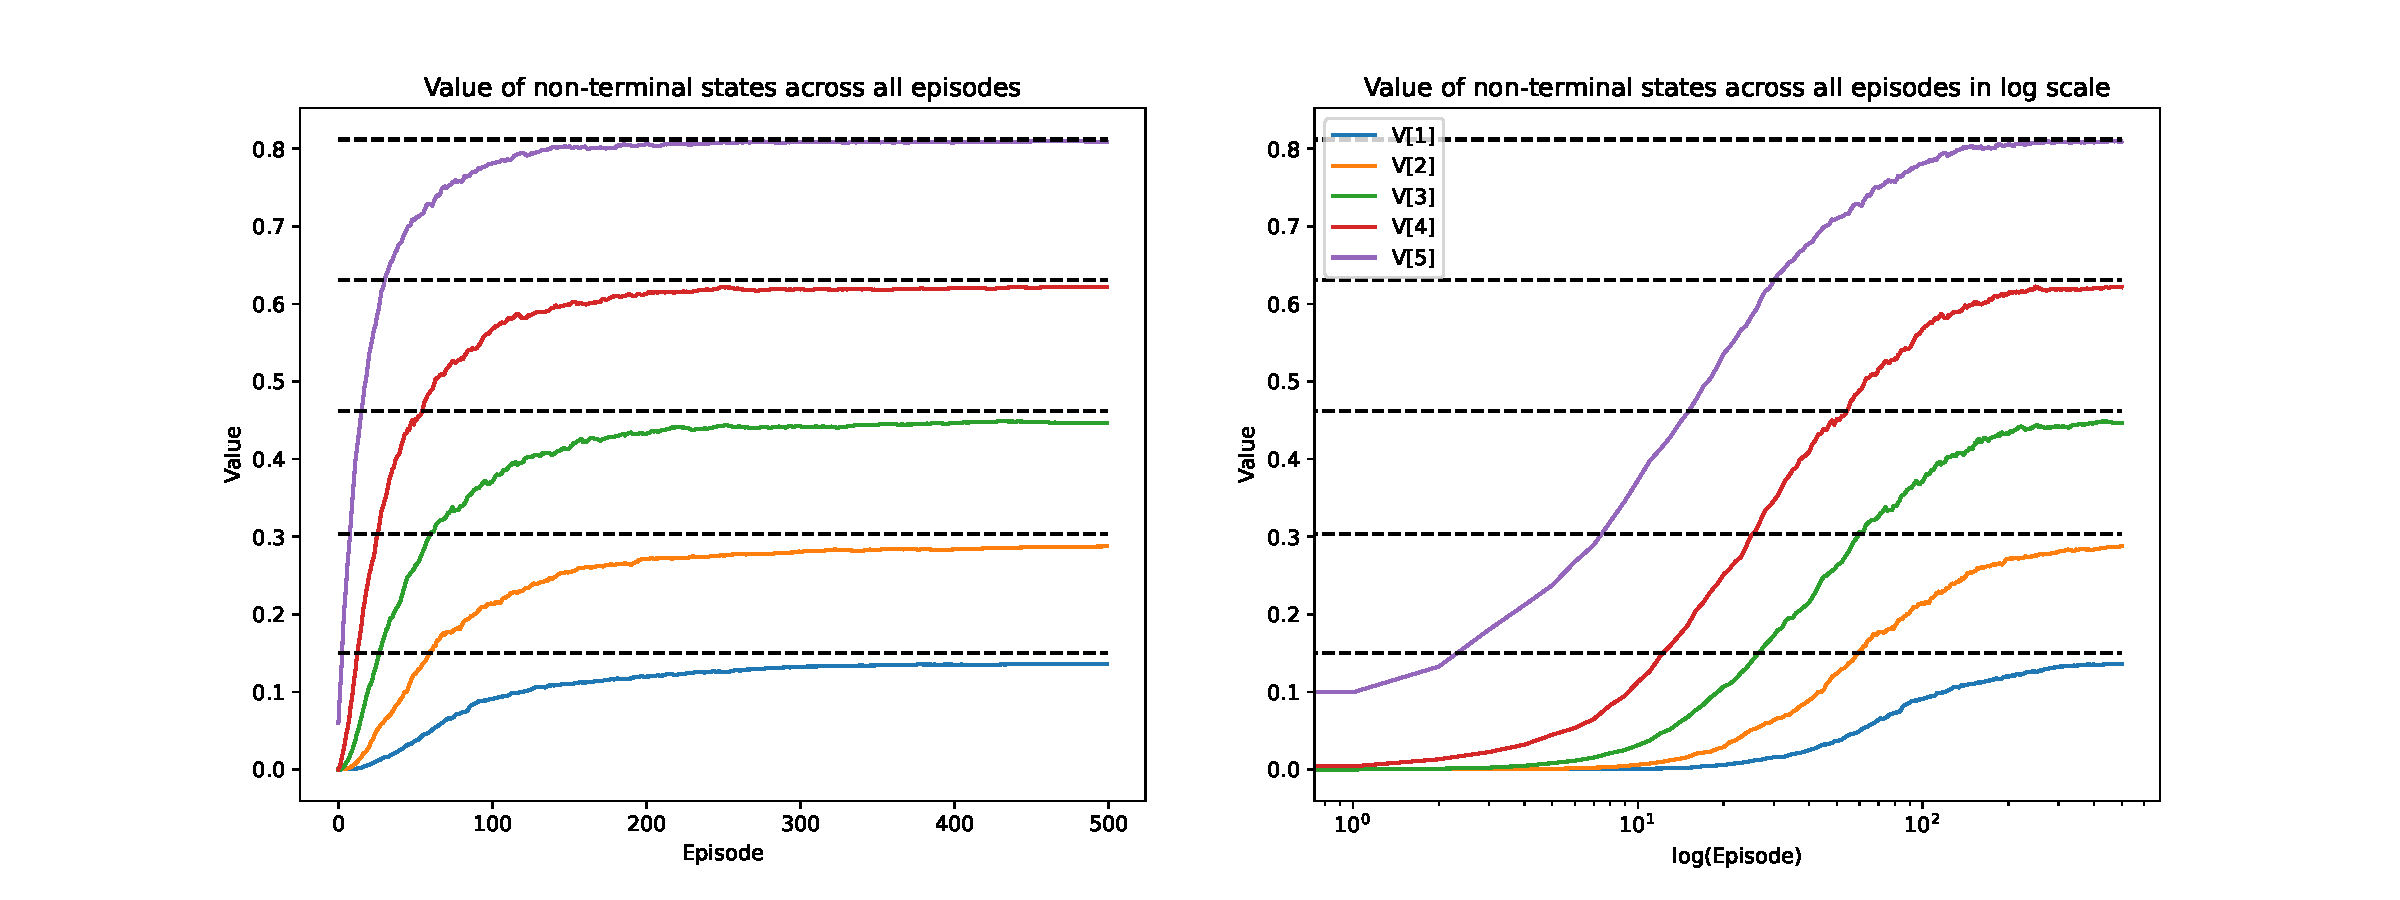
\includegraphics[width=\textwidth]{images/mc_td/td_experiments_50.pdf}
        \caption{Average state-values of 50 runs of TD with exponential decay and tuned hyperparameters}
        \label{fig:average_td}
    \end{figure}
    
    \item \textbf{Comparision of FVMC, EVMC and TD based on state-value functions across episodes and log-scale of episodes:} We can see that the state-values for FVMC and EVMC converge to the true values but the state-values for TD learning do not converge to the true values. This is consistent with the general behaviours of the algorithms. The variance in the state-values for FVMC and EVMC is higher than TD learning but the bias in the state-values for TD learning is higher than FVMC and EVMC. The plot on log-scale helps us to zoom into the first few episodes and make a better judgement on the high variance phenomenon of Monte Carlo methods.
    \item \textbf{Comparision of FVMC, EVMC and TD based on average target value for state 3:} We can see that the average across episodes for FVMC and EVMC osciilates between 0 and 1 but the average for TD learning has fewer oscillations but does not land at the true values. Thus, this is another view to note the high variance in Monte Carlo methods and the high bias in TD learning.

\end{enumerate}


\end{document}